% !TEX root = ../main.tex

\chapter{Appendix}
\label{appendix:dataAppendix}

The appendix contains extensions upon the information in the rest of the text. However, this information was not necessary to reach the desired conclusions in the text.

\section{Descriptive Statistics}
\label{appendix:descriptiveStatistics}

\subsection{Closing Prices}

\subsubsection{Entire Dataset}

\begin{figure}[h!]
\centering
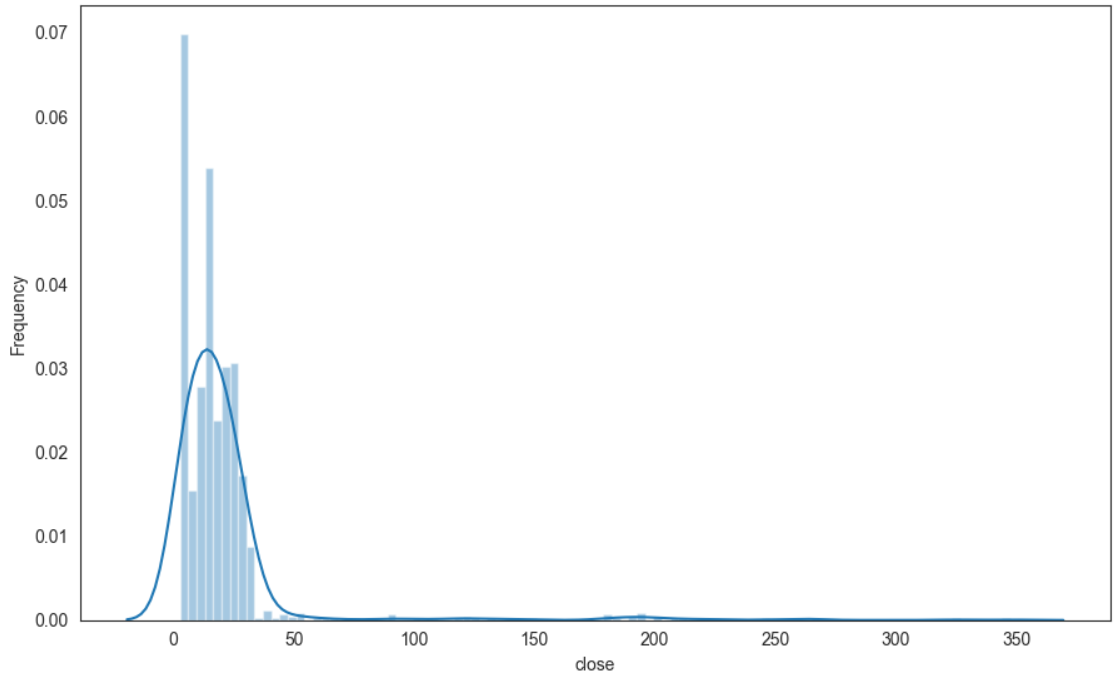
\includegraphics[width=15cm,height=7cm,keepaspectratio]{resultsEvaluation/closeDescMax.png}
\caption{Closing Prices with entire dataset}
\label{fig:appendix_closeDescMax}
\end{figure}
\begin{center}
\begin{tabular}{ c c }
\hline
\multicolumn{2}{|c|}{Closing Price Descriptive Statistics with entire dataset} \\
\hline
Mean & 20.25539316918189 \\
Standard Error & 0.8617871146224114 \\
Median & 15.22 \\
Mode & 4.14 \\
Standard Deviation & 30.56612021354625 \\
Sample Variance & 935.0303819398896 \\
Kurtosis & 43.00117239290764 \\
Skewness & 6.080884821536175 \\
Range & 344.71 \\
Minimum & 2.8 \\
Maximum & 347.51 \\
Sum & 25501.540000000005 \\
Count & 1259  
\end{tabular}
\end{center}

\subsubsection{Last Year}

\begin{figure}[h!]
\centering
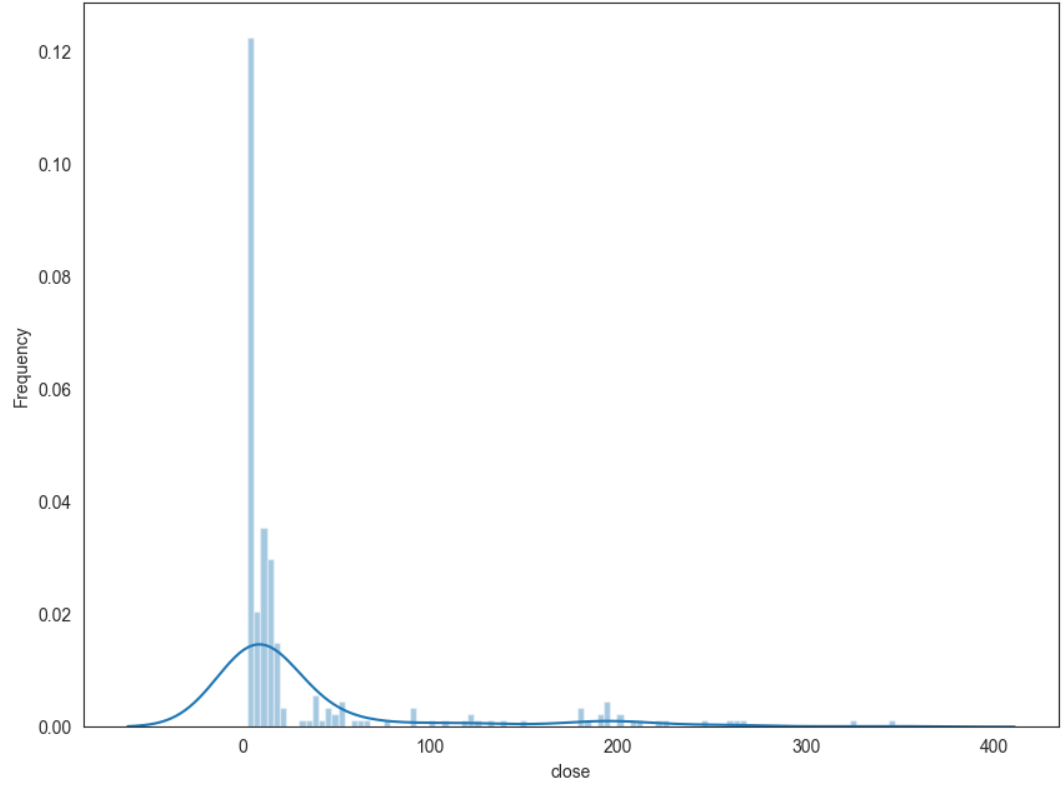
\includegraphics[width=15cm,height=7cm,keepaspectratio]{resultsEvaluation/closeDesc1.png}
\caption{Closing Prices in the last year of data}
\label{fig:appendix_closeDesc1}
\end{figure}
\begin{center}
\begin{tabular}{ c c }
\hline
\multicolumn{2}{|c|}{Closing Price Descriptive Statistics in the last year of data} \\
\hline
Mean & 35.32043478260869 \\
Standard Error & 4.034091200037088 \\
Median & 10.02 \\
Mode & 4.44 \\
Standard Deviation & 64.03921248871352 \\
Sample Variance & 4117.294627984817 \\
Kurtosis & 6.11122201031286 \\
Skewness & 2.5837008559997834 \\
Range & 344.71 \\
Minimum & 2.8 \\
Maximum & 347.51 \\
Sum & 8936.07 \\
Count & 253
\end{tabular}
\end{center}

\subsection{Trading Volume}

\subsubsection{Entire Dataset}

\begin{figure}[h!]
\centering
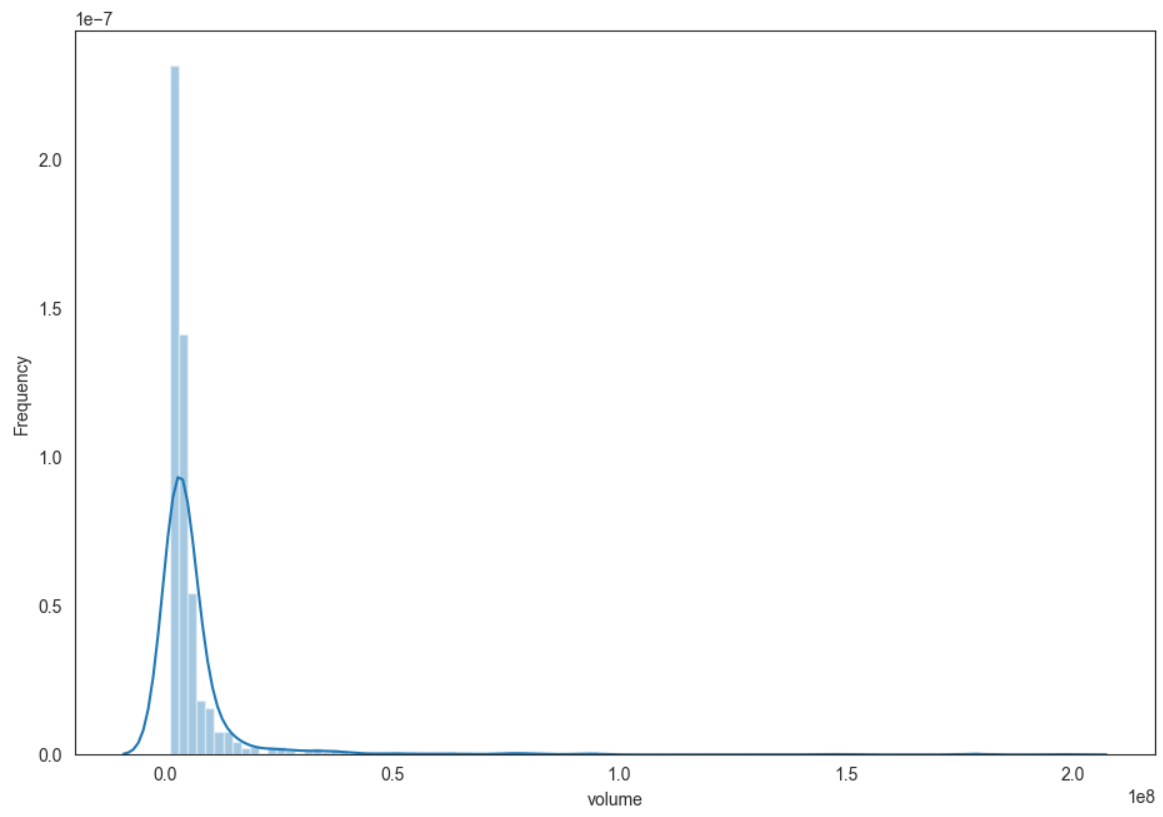
\includegraphics[width=15cm,height=7cm,keepaspectratio]{resultsEvaluation/volumeDescMax.png}
\caption{Trading Volume with entire dataset}
\label{fig:appendix_volumeDescMax}
\end{figure}
\begin{center}
\begin{tabular}{ c c }
\hline
\multicolumn{2}{|c|}{Trading Volume Descriptive Statistics with entire dataset} \\
\hline
Mean & 6435867.801429706 \\
Standard Error & 399372.9943423072 \\
Median & 3130713 \\
Mode & 1491760 \\
Standard Deviation & 14165079.458700724 \\
Sample Variance & 200808974859915.2 \\
Kurtosis & 81.30752829995787 \\
Skewness & 8.021781388564962 \\
Range & 196185042 \\
Minimum & 972904 \\
Maximum & 197157946 \\
Sum & 8102757562 \\
Count & 1259
\end{tabular}
\end{center}

\subsubsection{Last Year}

\begin{figure}[h!]
\centering
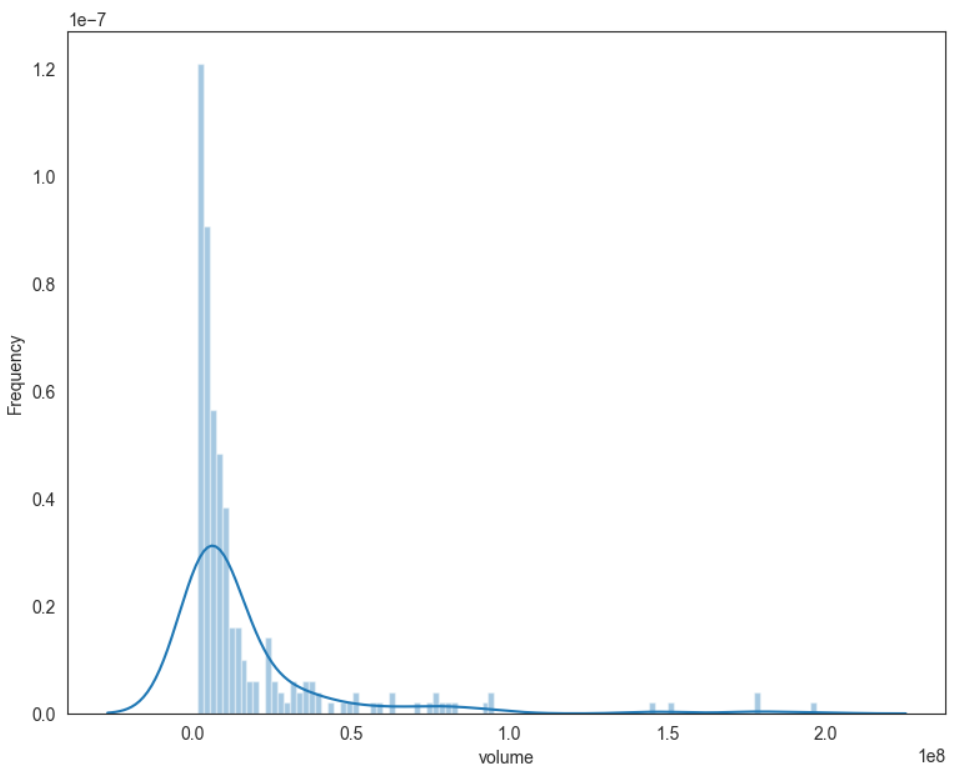
\includegraphics[width=15cm,height=7cm,keepaspectratio]{resultsEvaluation/volumeDesc1.png}
\caption{Trading Volume in the last year of data}
\label{fig:appendix_volumeDesc1}
\end{figure}
\begin{center}
\begin{tabular}{ c c }
\hline
\multicolumn{2}{|c|}{Trading Volume Descriptive Statistics in the last year of data} \\
\hline
Mean & 16731690.841897232 \\
Standard Error & 1798626.81876273 \\
Median & 6603951 \\
Mode & 4568695 \\
Standard Deviation & 28552315.58314456 \\
Sample Variance & 818469783592652.2 \\
Kurtosis & 16.215823114980463 \\
Skewness & 3.730320402302758 \\
Range & 195827485 \\
Minimum & 1330461 \\
Maximum & 197157946 \\
Sum & 4233117783 \\
Count & 253
\end{tabular}
\end{center}

\subsection{1 Day Returns}

\subsubsection{Entire Dataset}

\begin{figure}[h!]
\centering
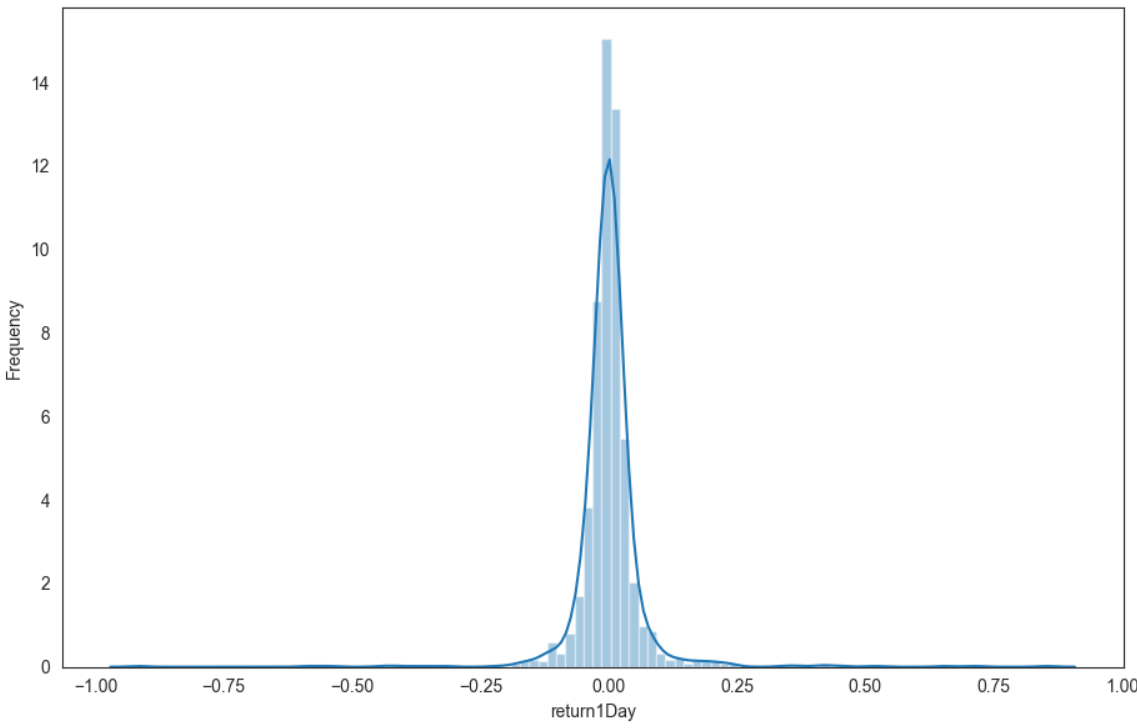
\includegraphics[width=15cm,height=7cm,keepaspectratio]{resultsEvaluation/1returnDescMax.png}
\caption{1 Day Returns with entire dataset}
\label{fig:appendix_1returnDescMax}
\end{figure}
\begin{center}
\begin{tabular}{ c c }
\hline
\multicolumn{2}{|c|}{1 Day Return Descriptive Statistics with entire dataset} \\
\hline
Mean & 0.0014490461774454091 \\
Standard Error & 0.0021291609999713954 \\
Median & 0.0 \\
Mode & 0.0 \\
Standard Deviation & 0.07548769098797223 \\
Sample Variance & 0.005702924817259385 \\
Kurtosis & 51.56501043384626 \\
Skewness & 0.7637560467880287 \\
Range & 1.770007043945965 \\
Minimum & -0.916290731874155 \\
Maximum & 0.85371631207181 \\
Sum & 1.8229000912263227 \\
Count & 1258
\end{tabular}
\end{center}

\subsubsection{Last Year}

\begin{figure}[h!]
\centering
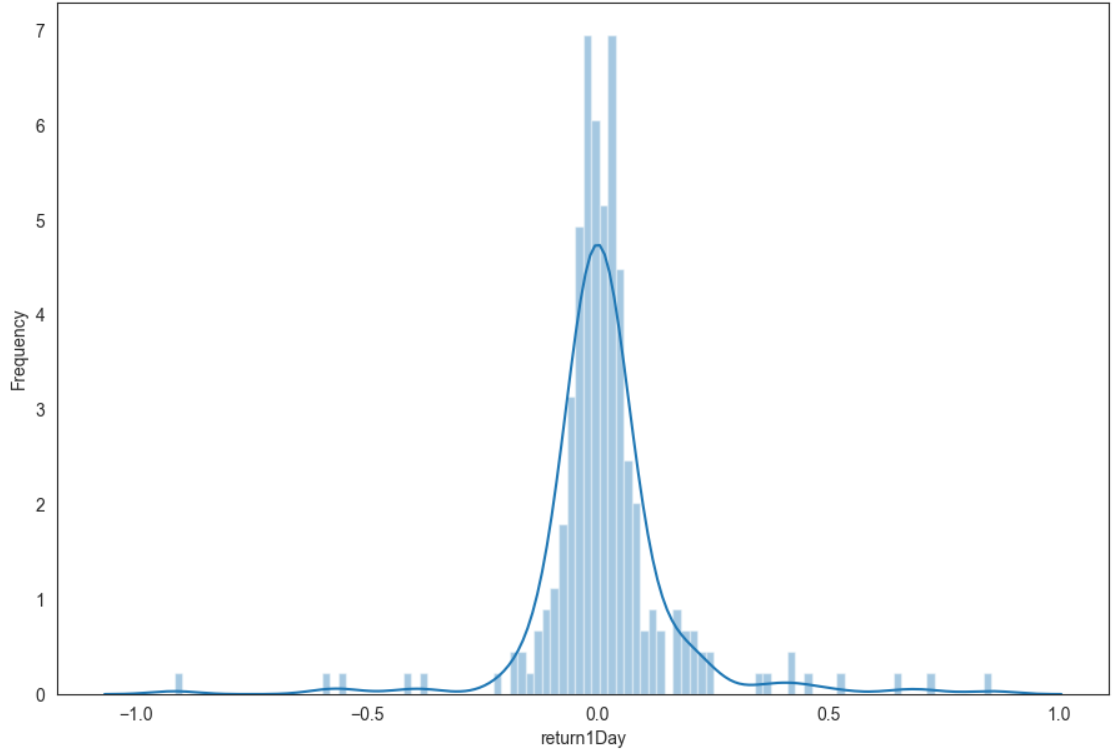
\includegraphics[width=15cm,height=7cm,keepaspectratio]{resultsEvaluation/1returnDesc1.png}
\caption{1 Day Returns in the last year of data}
\label{fig:appendix_1returnDesc1}
\end{figure}
\begin{center}
\begin{tabular}{ c c }
\hline
\multicolumn{2}{|c|}{1 Day Return Descriptive Statistics in the last year of data} \\
\hline
Mean & 0.01617449079992721 \\
Standard Error & 0.009609836418644279 \\
Median & 0.005313187705878563 \\
Mode & 0.022335953942063298 \\
Standard Deviation & 0.15224844154955602 \\
Sample Variance & 0.02327193691026168 \\
Kurtosis & 12.867982373920272 \\
Skewness & 0.32394336153811276 \\
Range & 1.770007043945965 \\
Minimum & -0.916290731874155 \\
Maximum & 0.85371631207181 \\
Sum & 4.075971681581655 \\
Count & 252
\end{tabular}
\end{center}

\subsection{Article Volume}

\subsubsection{Entire Dataset}

\begin{figure}[h!]
\centering
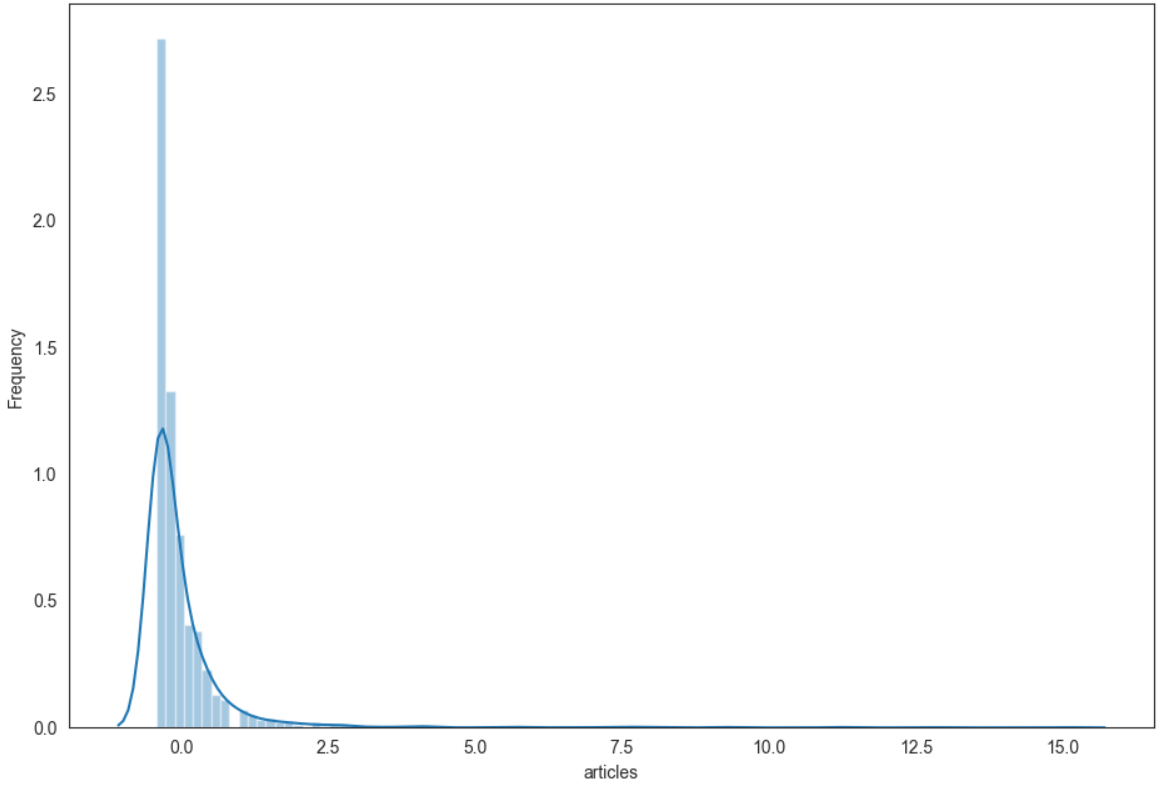
\includegraphics[width=15cm,height=7cm,keepaspectratio]{resultsEvaluation/articleDescMax.png}
\caption{Article Volume with entire dataset}
\label{fig:appendix_articleDescMax}
\end{figure}
\begin{center}
\begin{tabular}{ c c }
\hline
\multicolumn{2}{|c|}{Article Volume Descriptive Statistics with entire dataset} \\
\hline
Mean & -2.2065213996409285e-17 \\
Standard Error & 0.02196873875818734 \\
Median & -0.2421631034547878 \\
Mode & -0.41805802758295 \\
Standard Deviation & 1.0 \\
Sample Variance & 1.0004826254826256 \\
Kurtosis & 73.76924857053827 \\
Skewness & 7.360900854018193 \\
Range & 15.478753323278276 \\
Minimum & -0.41805802758295 \\
Maximum & 15.060695295695327 \\
Sum & -4.642022877199281e-12 \\
Count & 2073
\end{tabular}
\end{center}

\subsubsection{Last Year}

\begin{figure}[h!]
\centering
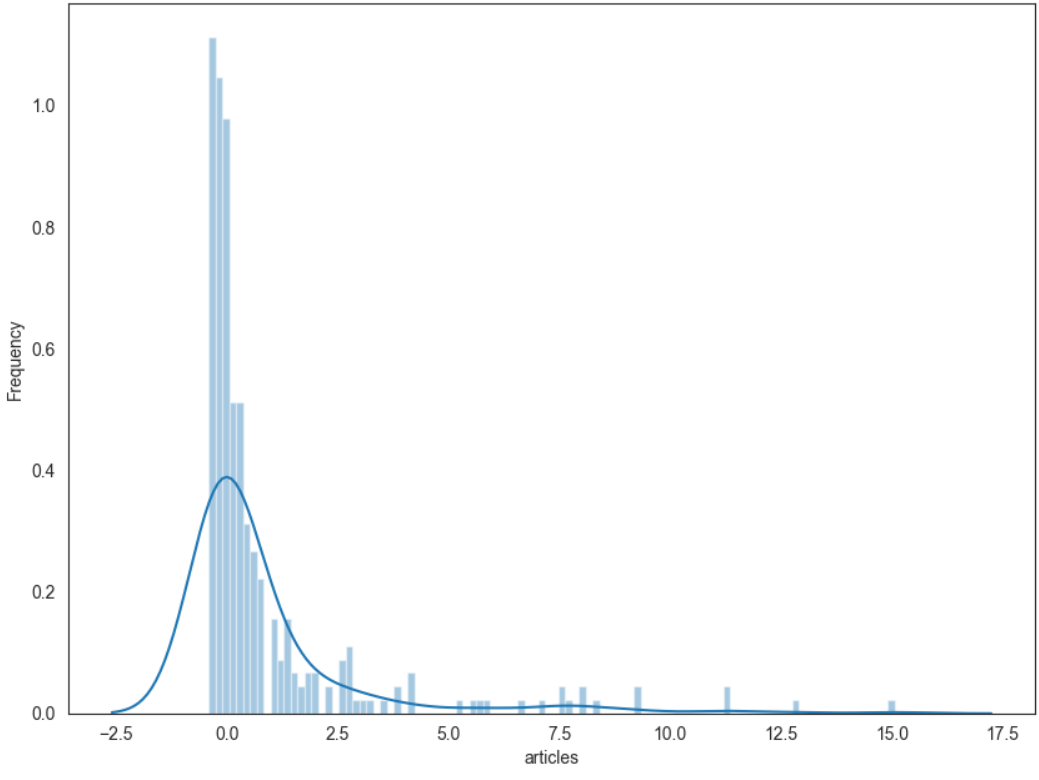
\includegraphics[width=15cm,height=7cm,keepaspectratio]{resultsEvaluation/articleDesc1.png}
\caption{Article Volume in the last year of data}
\label{fig:appendix_articleDesc1}
\end{figure}
\begin{center}
\begin{tabular}{ c c }
\hline
\multicolumn{2}{|c|}{Article Volume Descriptive Statistics in the last year of data} \\
\hline
Mean & 0.8623357132258448 \\
Standard Error & 0.1325148497318309 \\
Median & 0.1096267448015367 \\
Mode & -0.41805802758295 \\
Standard Deviation & 2.2527524454411254 \\
Sample Variance & 5.092453765840419 \\
Kurtosis & 12.21615870052046 \\
Skewness & 3.296079615884022 \\
Range & 15.478753323278276 \\
Minimum & -0.41805802758295 \\
Maximum & 15.060695295695327 \\
Sum & 250.07735683549507 \\
Count & 290
\end{tabular}
\end{center}

\subsection{Words Volume}

\subsubsection{Entire Dataset}

\begin{figure}[h!]
\centering
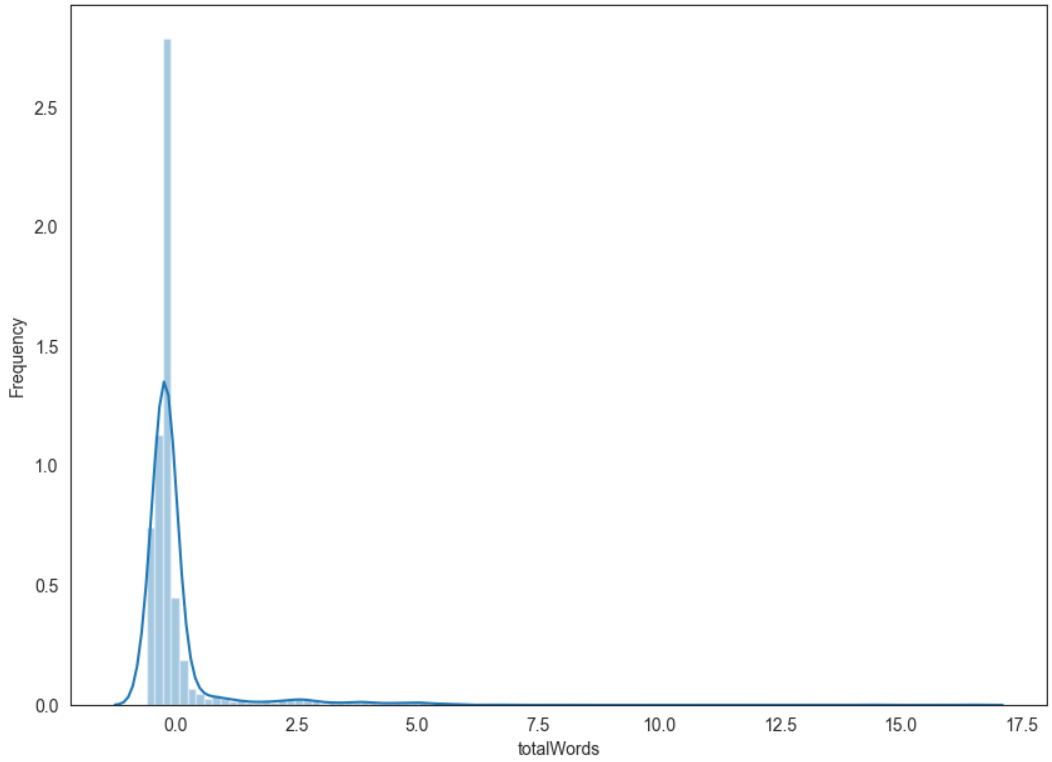
\includegraphics[width=15cm,height=7cm,keepaspectratio]{resultsEvaluation/wordsDescMax.png}
\caption{Words Volume with entire dataset}
\label{fig:appendix_wordsDescMax}
\end{figure}
\begin{center}
\begin{tabular}{ c c }
\hline
\multicolumn{2}{|c|}{Words Volume Descriptive Statistics with entire dataset} \\
\hline
Mean & 0.00013989387361311993 \\
Standard Error & 0.021968180574674083 \\
Median & -0.2 \\
Mode & -0.19 \\
Standard Deviation & 0.999974591918116 \\
Sample Variance & 1.0004317854395641 \\
Kurtosis & 66.70204164146547 \\
Skewness & 6.45609886055835 \\
Range & 17.07 \\
Minimum & -0.61 \\
Maximum & 16.46 \\
Sum & 0.28999999999995796 \\
Count & 2073
\end{tabular}
\end{center}

\subsubsection{Last Year}

\begin{figure}[h!]
\centering
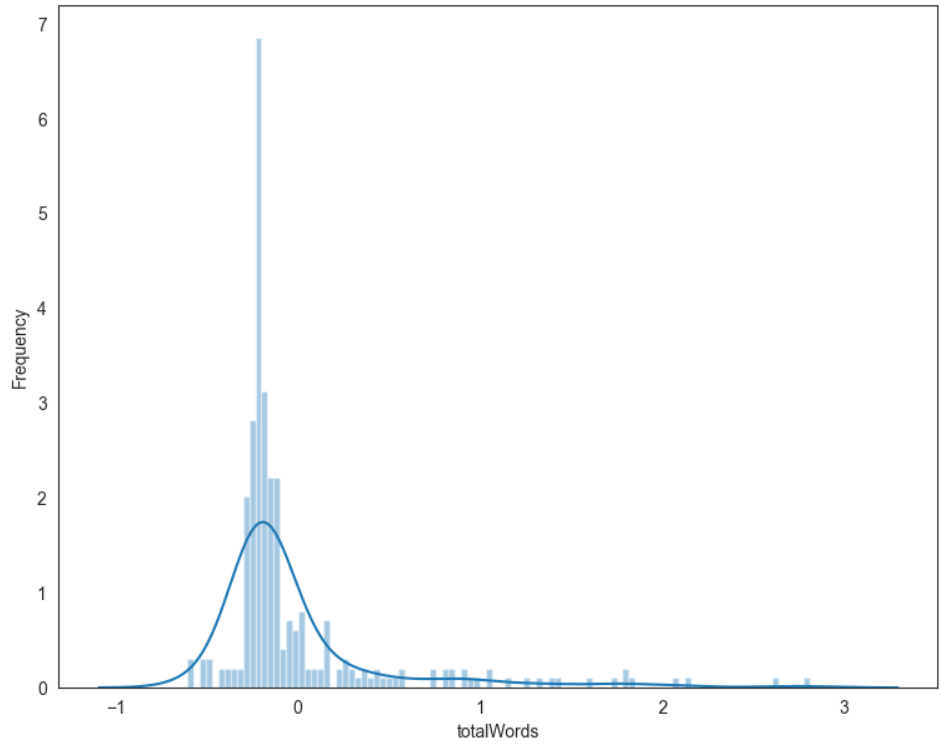
\includegraphics[width=15cm,height=7cm,keepaspectratio]{resultsEvaluation/wordsDesc1.png}
\caption{Words Volume in the last year of data}
\label{fig:appendix_wordsDesc1}
\end{figure}
\begin{center}
\begin{tabular}{ c c }
\hline
\multicolumn{2}{|c|}{Words Volume Descriptive Statistics in the last year of data} \\
\hline
Mean & -0.010758620689655175 \\
Standard Error & 0.029379055463608056 \\
Median & -0.19 \\
Mode & -0.22 \\
Standard Deviation & 0.4994439428813369 \\
Sample Variance & 0.2503073809807899 \\
Kurtosis & 9.61184972410166 \\
Skewness & 2.9411586965134755 \\
Range & 3.42 \\
Minimum & -0.61 \\
Maximum & 2.81 \\
Sum & -3.1200000000000068 \\
Count & 290
\end{tabular}
\end{center}

\subsection{Positive Sentiment}

\subsubsection{Entire Dataset}

\begin{figure}[h!]
\centering
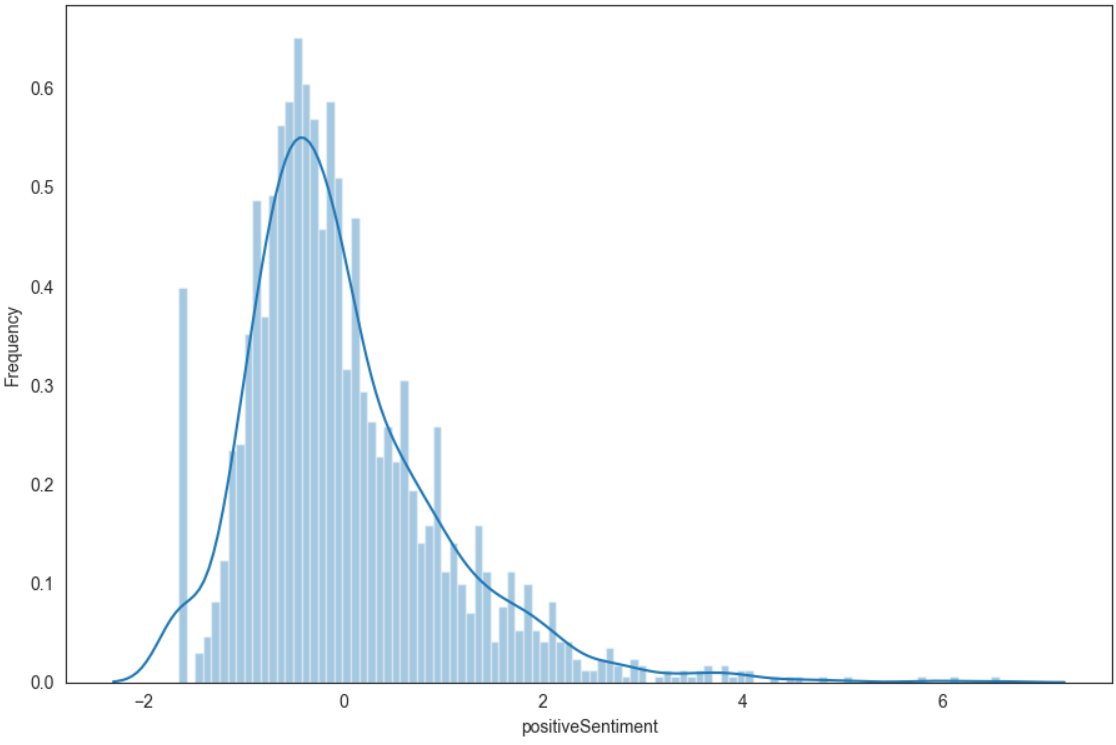
\includegraphics[width=15cm,height=7cm,keepaspectratio]{resultsEvaluation/positiveDescMax.png}
\caption{Positive Sentiment with entire dataset}
\label{fig:appendix_positiveDescMax}
\end{figure}
\begin{center}
\begin{tabular}{ c c }
\hline
\multicolumn{2}{|c|}{Positive Sentiment Descriptive Statistics with entire dataset} \\
\hline
Mean & -0.00011577424023154774 \\
Standard Error & 0.021969944580020426 \\
Median & -0.21 \\
Mode & -1.65 \\
Standard Deviation & 1.0000548880773885 \\
Sample Variance & 1.0005924576323273 \\
Kurtosis & 4.061676439612937 \\
Skewness & 1.4873401549309522 \\
Range & 8.22 \\
Minimum & -1.65 \\
Maximum & 6.57 \\
Sum & -0.23999999999965826 \\
Count & 2073
\end{tabular}
\end{center}

\subsubsection{Last Year}

\begin{figure}[h!]
\centering
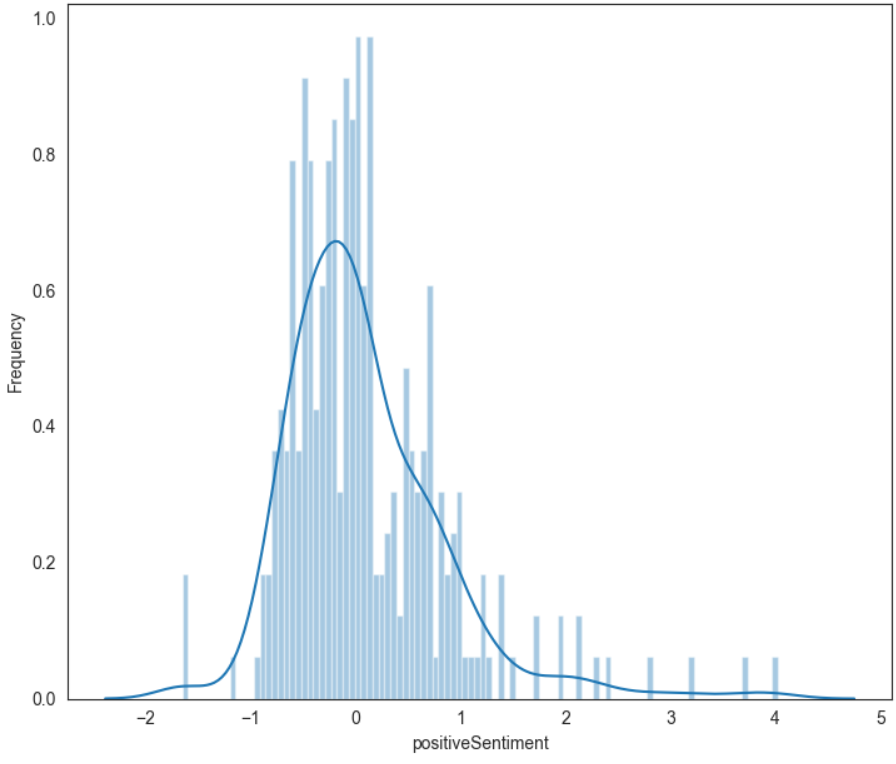
\includegraphics[width=15cm,height=7cm,keepaspectratio]{resultsEvaluation/positiveDesc1.png}
\caption{Positive Sentiment in the last year of data}
\label{fig:appendix_positiveDesc1}
\end{figure}
\begin{center}
\begin{tabular}{ c c }
\hline
\multicolumn{2}{|c|}{Positive Sentiment Descriptive Statistics in the last year of data} \\
\hline
Mean & 0.0863103448275862 \\
Standard Error & 0.04453127962901483 \\
Median & -0.055 \\
Mode & -0.1 \\
Standard Deviation & 0.7570317536932523 \\
Sample Variance & 0.5750801109652786 \\
Kurtosis & 5.009115638344465 \\
Skewness & 1.636685164397725 \\
Range & 5.67 \\
Minimum & -1.65 \\
Maximum & 4.02 \\
Sum & 25.029999999999973 \\
Count & 290
\end{tabular}
\end{center}

\subsection{Negative Sentiment}

\subsubsection{Entire Dataset}

\begin{figure}[h!]
\centering
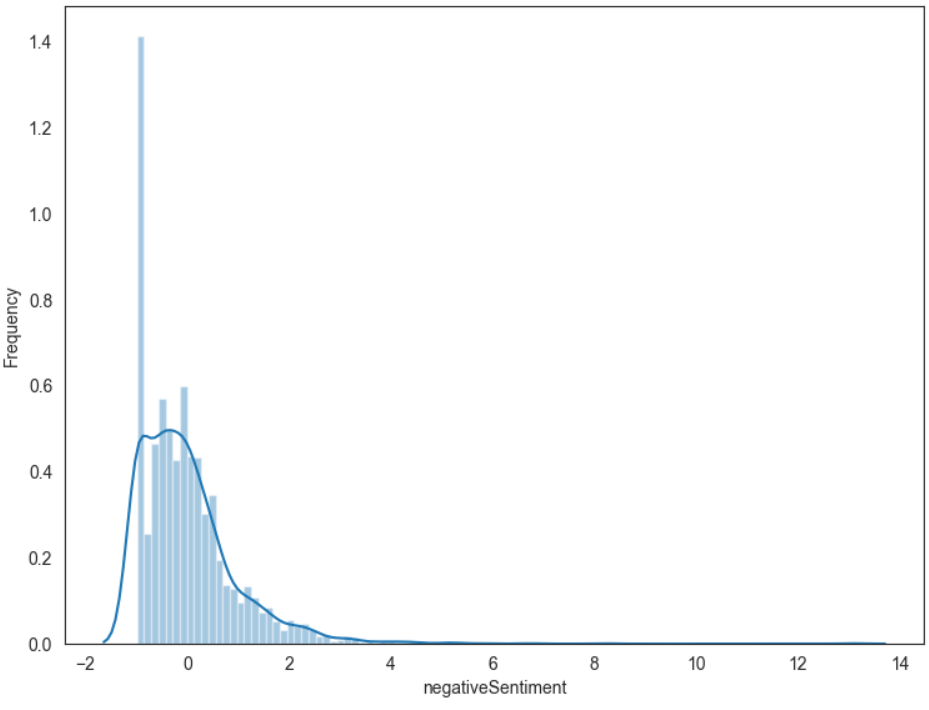
\includegraphics[width=15cm,height=7cm,keepaspectratio]{resultsEvaluation/negativeDescMax.png}
\caption{Negative Sentiment with entire dataset}
\label{fig:appendix_negativeDescMax}
\end{figure}
\begin{center}
\begin{tabular}{ c c }
\hline
\multicolumn{2}{|c|}{Negative Sentiment Descriptive Statistics with entire dataset} \\
\hline
Mean & 0.00014471780028943782 \\
Standard Error & 0.021964634770156394 \\
Median & -0.17 \\
Mode & -0.99 \\
Standard Deviation & 0.9998131896384166 \\
Sample Variance & 1.000108859355531 \\
Kurtosis & 19.513842113440127 \\
Skewness & 2.77912574439437 \\
Range & 14.05 \\
Minimum & -0.99 \\
Maximum & 13.06 \\
Sum & 0.30000000000174065 \\
Count & 2073
\end{tabular}
\end{center}

\subsubsection{Last Year}

\begin{figure}[h!]
\centering
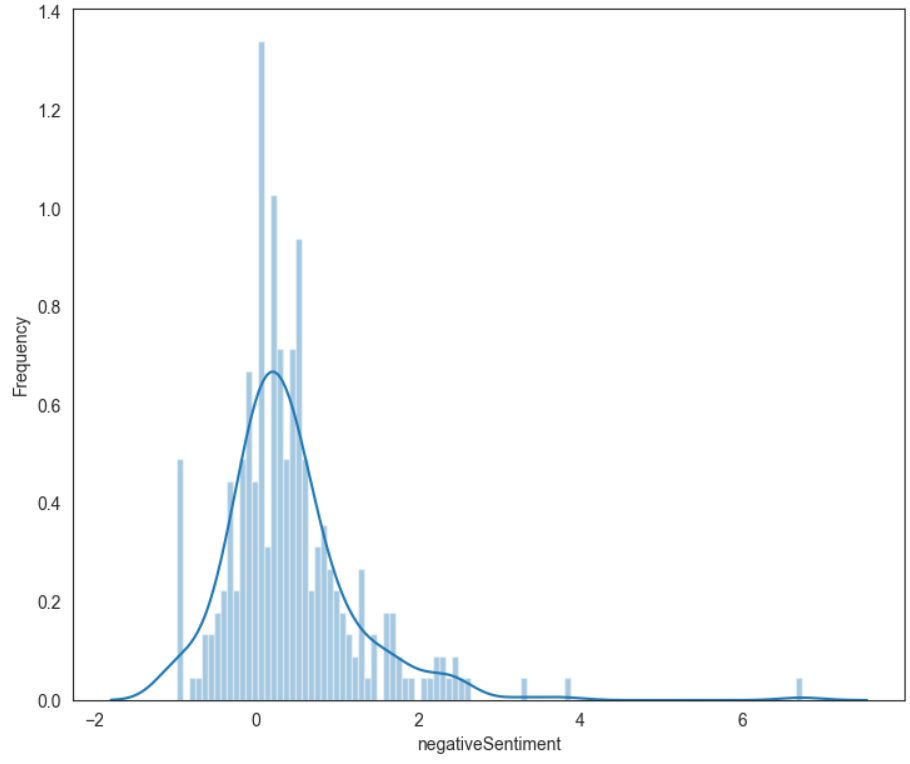
\includegraphics[width=15cm,height=7cm,keepaspectratio]{resultsEvaluation/negativeDesc1.png}
\caption{Negative Sentiment in the last year of data}
\label{fig:appendix_negativeDesc1}
\end{figure}
\begin{center}
\begin{tabular}{ c c }
\hline
\multicolumn{2}{|c|}{Negative Sentiment Descriptive Statistics in the last year of data} \\
\hline
Mean & 0.41293103448275864 \\
Standard Error & 0.04888104930864328 \\
Median & 0.27 \\
Mode & 0.08 \\
Standard Deviation & 0.8309778382469358 \\
Sample Variance & 0.6929135246390645 \\
Kurtosis & 11.895721323794636 \\
Skewness & 2.2637110757731076 \\
Range & 7.720000000000001 \\
Minimum & -0.99 \\
Maximum & 6.73 \\
Sum & 119.74999999999997 \\
Count & 290
\end{tabular}
\end{center}

\section{Auto-Correlation}
\label{appendix:autocorrelation}

\subsection{Closing Prices}

\begin{center}
\begin{tabular}{ c c c } 
\hline
\multicolumn{3}{|c|}{Closing Price AutoCorrelation with entire dataset} \\
\hline
Lag & Correlation & P-Value \\
\hline
1 & 0.9412 & 0.0 \\
2 & 0.9109 & 0.0 \\
3 & 0.8589 & 0.0 \\
4 & 0.7893 & 0.0 \\
5 & 0.7581 & 0.0 \\
\end{tabular}
\end{center}

\subsection{Trading Volume}

\begin{center}
\begin{tabular}{ c c c }
\hline
\multicolumn{3}{|c|}{Trading Volume AutoCorrelation with entire dataset} \\
\hline
Lag & Correlation & P-Value \\
\hline
1 & 0.7671 & 0.0 \\
2 & 0.6016 & 0.0 \\
3 & 0.5088 & 0.0 \\
4 & 0.4437 & 0.0 \\
5 & 0.4851 & 0.0 \\
\end{tabular}
\end{center}

\subsection{1 Day Returns}

\begin{center}
\begin{tabular}{ c c c }
\hline
\multicolumn{3}{|c|}{1 Day Return AutoCorrelation with entire dataset} \\
\hline
Lag & Correlation & P-Value \\
\hline
1 & 0.01 & 0.722 \\
2 & 0.1342 & 0.0 \\
3 & 0.1771 & 0.0 \\
4 & -0.2328 & 0.0 \\
5 & 0.0306 & 0.2795 \\
\end{tabular}
\end{center}

\subsection{Article Volume}

\begin{center}
\begin{tabular}{ c c c }
\hline
\multicolumn{3}{|c|}{Article Volume AutoCorrelation with entire dataset} \\
\hline
Lag & Correlation & P-Value \\
\hline
1 & 0.7087 & 0.0 \\
2 & 0.5052 & 0.0 \\
3 & 0.3913 & 0.0 \\
4 & 0.3588 & 0.0 \\
5 & 0.4346 & 0.0 \\
\end{tabular}
\end{center}

\subsection{Word Volume}

\begin{center}
\begin{tabular}{ c c c }
\hline
\multicolumn{3}{|c|}{Word Volume AutoCorrelation with entire dataset} \\
\hline
Lag & Correlation & P-Value \\
\hline
1 & 0.0512 & 0.0198 \\
2 & 0.0317 & 0.1497 \\
3 & 0.037 & 0.0927 \\
4 & 0.0106 & 0.6302 \\
5 & 0.0285 & 0.1947 \\
\end{tabular}
\end{center}

\subsection{Positive Sentiment}

\begin{center}
\begin{tabular}{ c c c }
\hline
\multicolumn{3}{|c|}{Positive Sentiment AutoCorrelation with entire dataset} \\
\hline
Lag & Correlation & P-Value \\
\hline
1 & 0.2189 & 0.0 \\
2 & 0.167 & 0.0 \\
3 & 0.1394 & 0.0 \\
4 & 0.1571 & 0.0 \\
5 & 0.1268 & 0.0 \\
\end{tabular}
\end{center}

\subsection{Negative Sentiment}

\begin{center}
\begin{tabular}{ c c c }
\hline
\multicolumn{3}{|c|}{Negative Sentiment AutoCorrelation with entire dataset} \\
\hline
Lag & Correlation & P-Value \\
\hline
1 & 0.1936 & 0.0 \\
2 & 0.1473 & 0.0 \\
3 & 0.1388 & 0.0 \\
4 & 0.1002 & 0.0 \\
5 & 0.1903 & 0.0 \\
\end{tabular}
\end{center}

\section{Return Vs Sentiment Correlation}
\label{appendix:returnSentimentCorrelation}

\subsection{1 Day Return Vs Negative Sentiment}

\begin{figure}[h!]
\centering
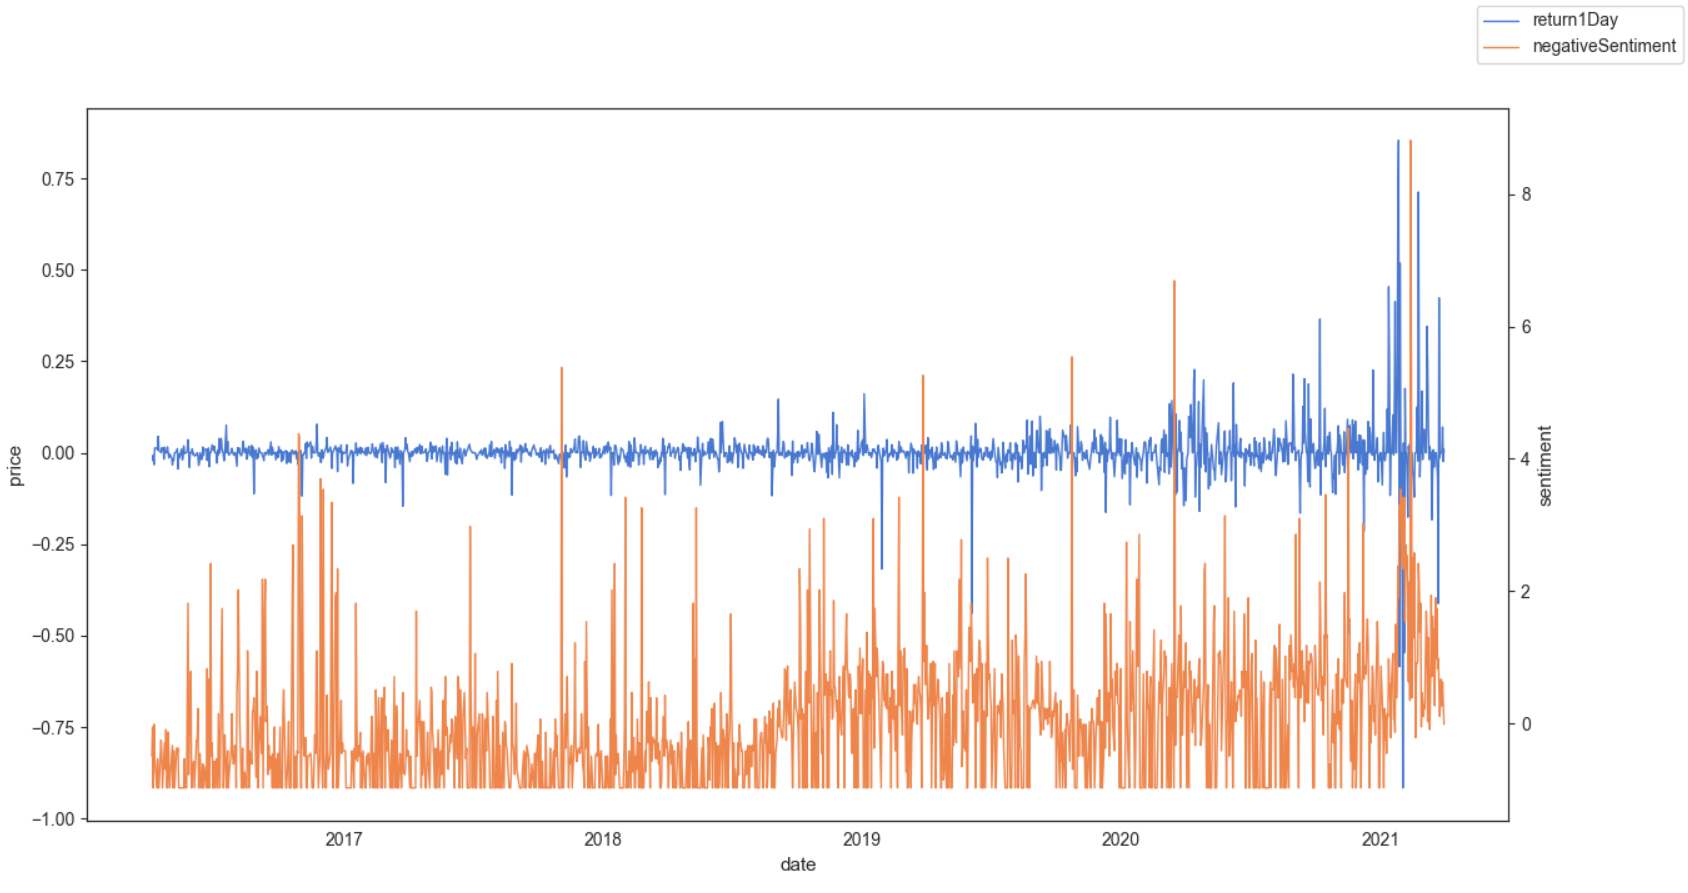
\includegraphics[width=15cm,height=7cm,keepaspectratio]{resultsEvaluation/1returnVsNeg.png}
\caption{1 Day Returns Vs Negative Sentiment with entire dataset}
\label{fig:appendix_1returnVsNeg}
\end{figure}

\begin{center}
\begin{tabular}{ c|c c|c c }
\hline
\multicolumn{5}{|c|}{1 Day Return Vs Negative Sentiment Correlation with entire dataset} \\
\hline
& \multicolumn{2}{|c|}{1 Day Return/Negative Sentiment} & \multicolumn{2}{|c }{Negative Sentiment/1 Day Return} \\
\hline
Lag & Correlation & P-Value & Correlation & P-Value \\
\hline
0 & -0.0057 & 0.8173 & -0.0057 & 0.8173 \\
1 & 0.0477 & 0.0554 & -0.0199 & 0.4249 \\
2 & 0.0318 & 0.2013 & -0.0186 & 0.4542 \\
3 & 0.0474 & 0.0571 & -0.0319 & 0.2002 \\
4 & -0.007 & 0.7782 & -0.0442 & 0.0757 \\
5 & 0.0431 & 0.0834 & -0.0444 & 0.0748 \\
\end{tabular}
\end{center}

\subsection{1 Day Return Vs Article Volume}

\begin{figure}[h!]
\centering
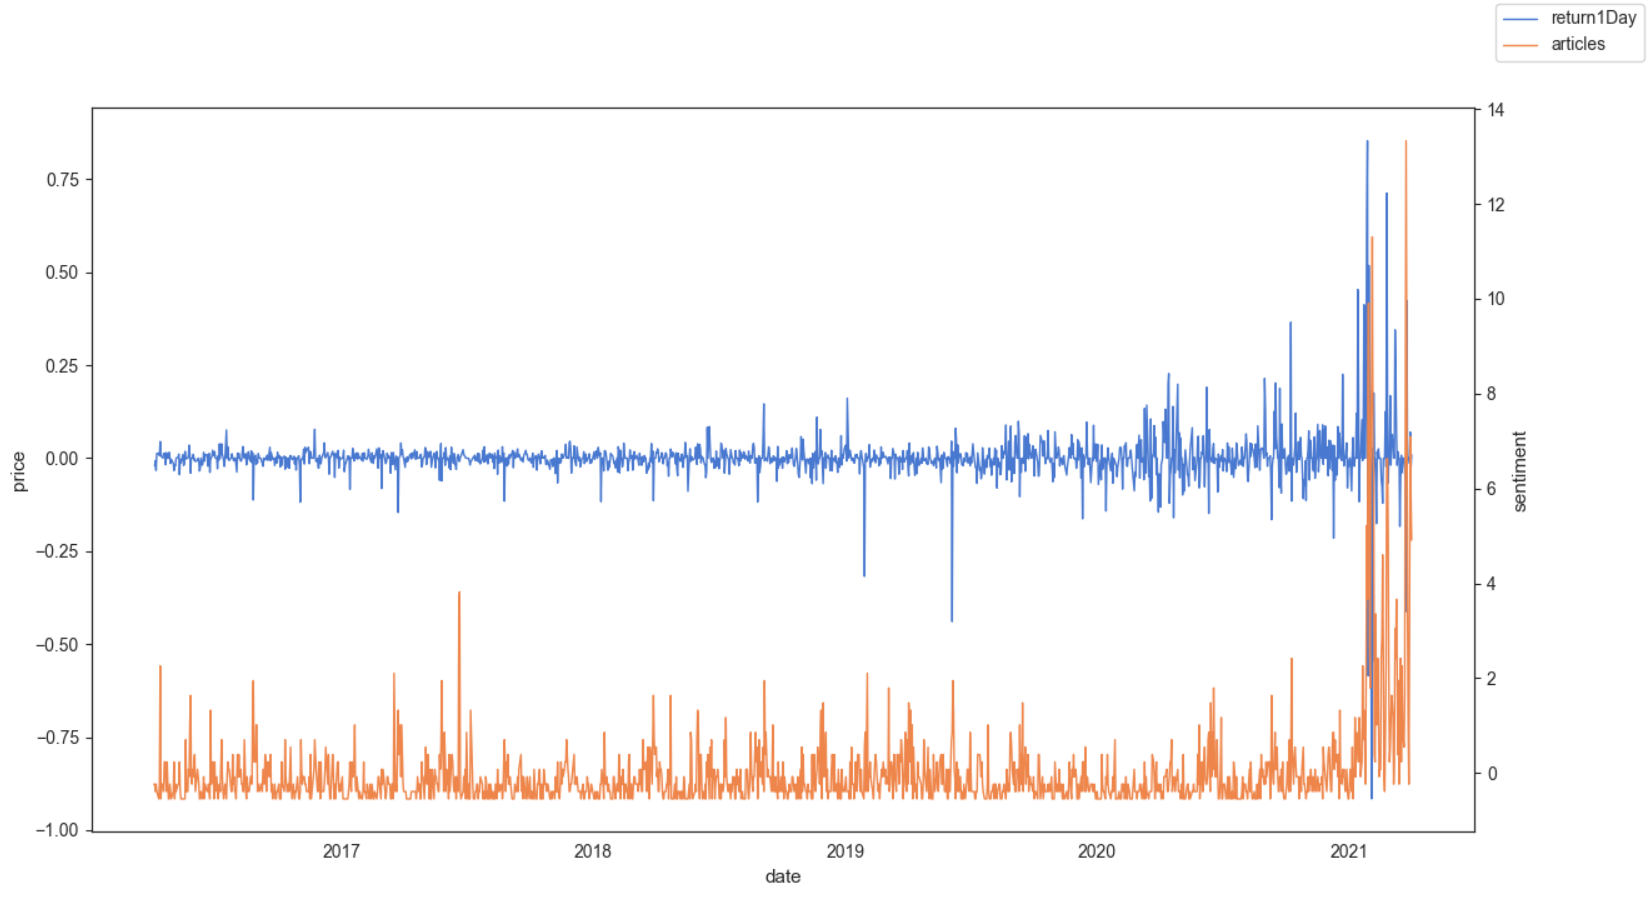
\includegraphics[width=15cm,height=7cm,keepaspectratio]{resultsEvaluation/1returnVsArticles.png}
\caption{1 Day Returns Vs Article Volume with entire dataset}
\label{fig:appendix_1returnVsArticle}
\end{figure}

\begin{center}
\begin{tabular}{ c|c c|c c }
\hline
\multicolumn{5}{|c|}{1 Day Return Vs Article Volume Correlation with entire dataset} \\
\hline
& \multicolumn{2}{|c|}{1 Day Return/Article Volume} & \multicolumn{2}{|c }{Article Volume/1 Day Return} \\
\hline
Lag & Correlation & P-Value & Correlation & P-Value \\
\hline
0 & -0.0316 & 0.2037 & -0.0316 & 0.2037 \\
1 & -0.0344 & 0.1674 & 0.019 & 0.4449 \\
2 & 0.0926 & 0.0002 & 0.0098 & 0.6924 \\
3 & 0.0749 & 0.0026 & -0.0354 & 0.1555 \\
4 & 0.0402 & 0.1066 & -0.07 & 0.0049 \\
5 & 0.1267 & 0.0 & -0.0679 & 0.0064 \\
\end{tabular}
\end{center}

\subsection{1 Day Return Vs Negative to Positive Sentiment Ratio}

\begin{figure}[h!]
\centering
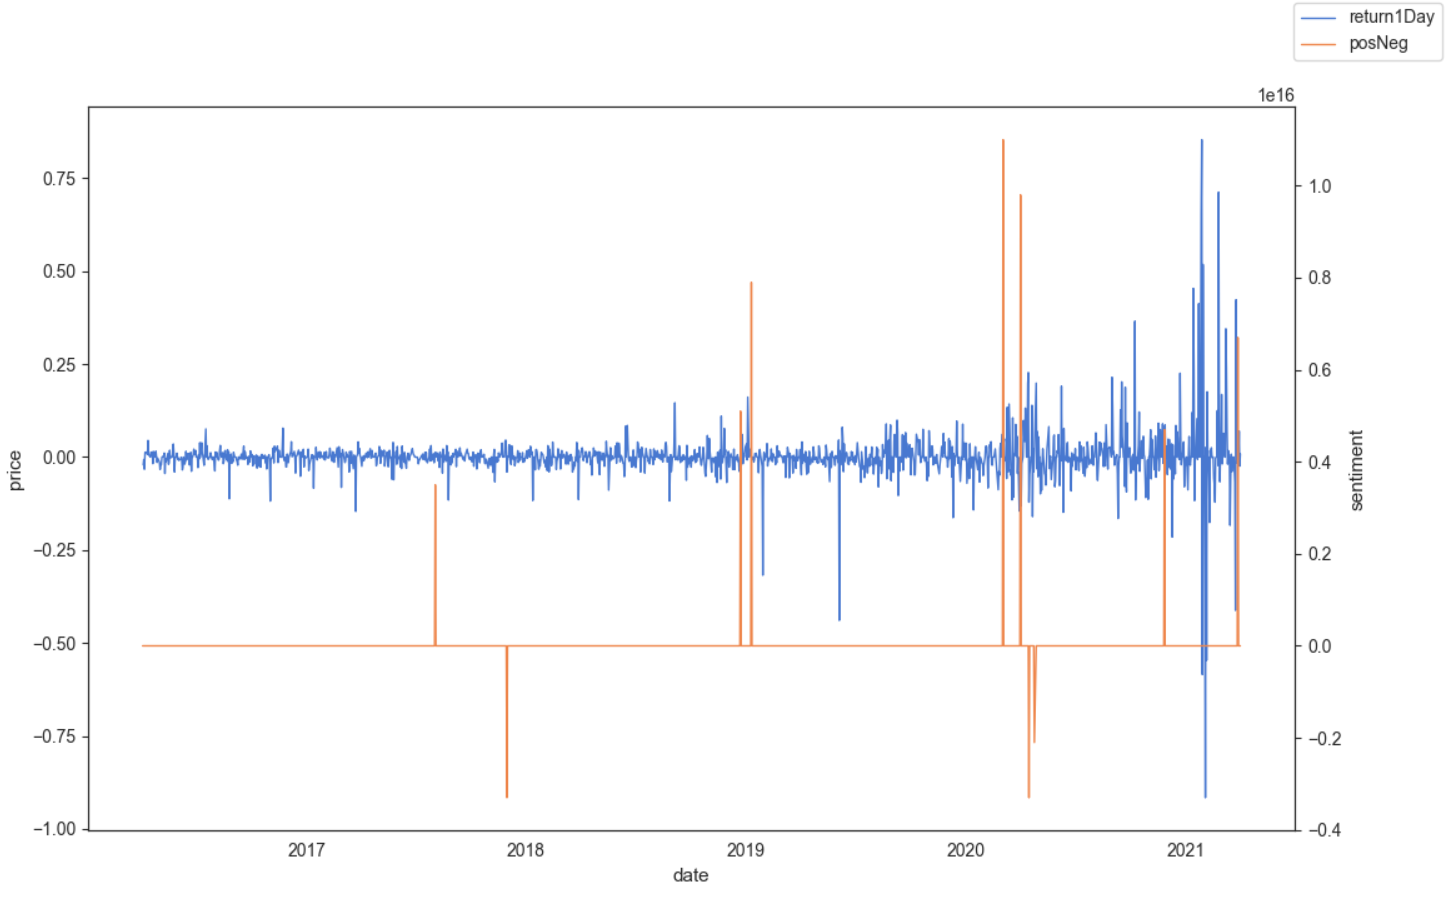
\includegraphics[width=15cm,height=7cm,keepaspectratio]{resultsEvaluation/1returnVsPosNeg.png}
\caption{1 Day Returns Vs Negative to Positive Sentiment Ratio with entire dataset}
\label{fig:appendix_1returnVsPosNeg}
\end{figure}

\begin{center}
\begin{tabular}{ c|c c|c c }
\hline
\multicolumn{5}{|c|}{1 Day Return Vs Negative to Positive Sentiment Ratio Correlation with entire dataset} \\
\hline
& \multicolumn{2}{|c|}{1 Day Return/Negative to Positive} & \multicolumn{2}{|c }{Negative to Positive/1 Day Return} \\
\hline
Lag & Correlation & P-Value & Correlation & P-Value \\
\hline
0 & -0.0152 & 0.5416 & -0.0152 & 0.5416 \\
1 & -0.0015 & 0.9513 & -0.0167 & 0.5031 \\
2 & -0.0476 & 0.0557 & 0.0177 & 0.4784 \\
3 & 0.0721 & 0.0038 & -0.0042 & 0.8674 \\
4 & -0.0615 & 0.0134 & 0.0187 & 0.4525 \\
5 & 0.0071 & 0.7761 & -0.0168 & 0.4997 \\
\end{tabular}
\end{center}

\section{Vector Autoregression}
\label{appendix:vectorAutoregression}

\subsection{1 Day Return, Positive Sentiment}

\subsubsection{Lag Selection}

\begin{center}
\begin{tabular}{ c c c c c c }
lags & loglik & p(LR) & AIC & BIC & HQC \\
\hline
1 & -167.03549 & & 0.215352 & 0.235447 & 0.222813 \\
2 & -145.69666 & 0.00000 & 0.193773 & 0.227265 & 0.206207 \\
3 & -144.93663 & 0.82308 & 0.197805 & 0.244694 & 0.215213 \\
4 & -142.65017 & 0.33399 & 0.199938 & 0.260223 & 0.222319 \\
5 & -123.75024 & 0.00000 & 0.181394 & 0.255076 & 0.208749 \\
\arrayrulecolor{red}\hline
6 & -64.95396 & 0.00000 & 0.113197 & 0.200276 & 0.145525 \\
\arrayrulecolor{red}\hline
7 & -63.78198 & 0.67278 & 0.116717 & 0.217192 & 0.154018 \\
8 & -63.68900 & 0.99594 & 0.121579 & 0.235451 & 0.163855 \\
9 & -58.31330 & 0.02950 & 0.119867 & 0.247136 & 0.167116 \\
10 & -56.14951 & 0.36349 & 0.122152 & 0.262818 & 0.174375 \\
\end{tabular}
\end{center}

\subsubsection{Unit Root Test}

\paragraph{1 Day Return}

Augmented Dickey-Fuller test for return1Day
testing down from 6 lags, criterion AIC
sample size 1611
unit-root null hypothesis: a = 1

test with constant 
including 5 lags of (1-L)return1Day
model: (1-L)y = b0 + (a-1)*y(-1) + ... + e
estimated value of (a - 1): -0.917446
test statistic: tau\_c(1) = -17.9067
asymptotic p-value 5.185e-043
1st-order autocorrelation coeff. for e: 0.007
lagged differences: F(5, 1604) = 32.364 [0.0000]

\paragraph{Positive Sentiment}

Augmented Dickey-Fuller test for positiveSentiment
testing down from 6 lags, criterion AIC
sample size 1612
unit-root null hypothesis: a = 1

test with constant 
including 5 lags of (1-L)positiveSentiment
model: (1-L)y = b0 + (a-1)*y(-1) + ... + e
estimated value of (a - 1): -0.535408
test statistic: tau\_c(1) = -12.0745
asymptotic p-value 5.969e-026
1st-order autocorrelation coeff. for e: -0.002
lagged differences: F(5, 1605) = 9.252 [0.0000]

\subsubsection{Vector Autoregression}

\begin{center}
VAR system, lag order 6\\
OLS estimates, observations 2016-04-13--2022-06-15 ($T=1611$)
\end{center}
\noindent
Log-likelihood = $-$62.7906\par
\noindent
Determinant of covariance matrix = 0.00370600\par
\noindent
AIC $= 0.1102$ \par
\noindent
BIC $= 0.1971$ \par
\noindent
HQC $= 0.1425$ \par
\noindent
Portmanteau test: LB(48) = 340.694, df = 168 [0.0000]\par
\begin{center}

Equation 1: return1Day\\

\begin{longtable}{lr@{.}lr@{.}lr@{.}lr@{.}l}
    \hline
    &
    \multicolumn{2}{c}{Coefficient} &
    \multicolumn{2}{c}{Std.\ Error} &
    \multicolumn{2}{c}{$t$-ratio} &
    \multicolumn{2}{c}{p-value} \\
    \hline
    \endfirsthead
    \multicolumn{4}{c}%
    {\tablename\ \thetable\ -- \textit{Continued from previous page}} \\
    \hline
    &
    \multicolumn{2}{c}{Coefficient} &
    \multicolumn{2}{c}{Std.\ Error} &
    \multicolumn{2}{c}{$t$-ratio} &
    \multicolumn{2}{c}{p-value} \\
    \hline
    \endhead
    \hline \multicolumn{4}{r}{\textit{Continued on next page}} \\
    \endfoot
    \hline
    \endlastfoot
const &
    0&00104449 &
    0&00158960 &
        0&6571 &
        0&5112 \\
return1Day$_{t-1}$ &
    0&0532996 &
    0&0242004 &
        2&202 &
        0&0278 \\
return1Day$_{t-2}$ &
    0&120869 &
    0&0240410 &
        5&028 &
        0&0000 \\
return1Day$_{t-3}$ &
    0&00536865 &
    0&0242304 &
        0&2216 &
        0&8247 \\
return1Day$_{t-4}$ &
    0&0291020 &
    0&0242268 &
        1&201 &
        0&2298 \\
return1Day$_{t-5}$ &
    0&124562 &
    0&0240438 &
        5&181 &
        0&0000 \\
return1Day$_{t-6}$ &
    $-$0&253442 &
    0&0242196 &
        $-$10&46 &
        0&0000 \\
positiveSentiment\_1 &
    0&000327211 &
    0&00165166 &
        0&1981 &
        0&8430 \\
positiveSentiment\_2 &
    0&00166040 &
    0&00167586 &
        0&9908 &
        0&3219 \\
positiveSentiment\_3 &
    $-$0&000924404 &
    0&00168180 &
        $-$0&5497 &
        0&5826 \\
positiveSentiment\_4 &
    0&000692590 &
    0&00168187 &
        0&4118 &
        0&6805 \\
positiveSentiment\_5 &
    0&00110231 &
    0&00167603 &
        0&6577 &
        0&5108 \\
positiveSentiment\_6 &
    $-$0&000182041 &
    0&00165063 &
        $-$0&1103 &
        0&9122 \\
\end{longtable}

\begin{tabular}{lrlr}
Mean dependent var &  0.001149 & S.D. dependent var &  0.066721 \\
Sum squared resid &  6.496350 & S.E. of regression &  0.063760 \\
$R^2$ &  0.093595 & Adjusted $R^2$ &  0.086788 \\
$F(12, 1598)$ &  13.75066 & P-value($F$) &  1.68\textrm{e--27} \\
$\hat{\rho}$ &  0.006756 & Durbin--Watson &  1.986226 \\
\end{tabular}

\end{center}

\begin{center}
F-tests of zero restrictions\\[1em]
\begin{tabular}{lll}
All lags of return1Day & $F(6, 1598) = 27.2175$ & [0.0000]\\
All lags of positiveSentiment & $F(6, 1598) = 0.342766$ & [0.9143]\\
All vars, lag 6 & $F(2, 1598) = 54.7514$ & [0.0000]\\
\end{tabular}
\end{center}

\begin{center}

Equation 2: positiveSentiment\\

\begin{longtable}{lr@{.}lr@{.}lr@{.}lr@{.}l}
    \hline
    &
    \multicolumn{2}{c}{Coefficient} &
    \multicolumn{2}{c}{Std.\ Error} &
    \multicolumn{2}{c}{$t$-ratio} &
    \multicolumn{2}{c}{p-value} \\
    \hline
    \endfirsthead
    \multicolumn{4}{c}%
    {\tablename\ \thetable\ -- \textit{Continued from previous page}} \\
    \hline
    &
    \multicolumn{2}{c}{Coefficient} &
    \multicolumn{2}{c}{Std.\ Error} &
    \multicolumn{2}{c}{$t$-ratio} &
    \multicolumn{2}{c}{p-value} \\
    \hline
    \endhead
    \hline \multicolumn{4}{r}{\textit{Continued on next page}} \\
    \endfoot
    \hline
    \endlastfoot
const &
    0&00140979 &
    0&0239976 &
        0&05875 &
        0&9532 \\
return1Day$_{t-1}$ &
    0&286432 &
    0&365343 &
        0&7840 &
        0&4332 \\
return1Day$_{t-2}$ &
    0&231605 &
    0&362937 &
        0&6381 &
        0&5235 \\
return1Day$_{t-3}$ &
    $-$0&00497079 &
    0&365796 &
        $-$0&01359 &
        0&9892 \\
return1Day$_{t-4}$ &
    0&0475274 &
    0&365742 &
        0&1299 &
        0&8966 \\
return1Day$_{t-5}$ &
    0&428067 &
    0&362979 &
        1&179 &
        0&2384 \\
return1Day$_{t-6}$ &
    0&219204 &
    0&365634 &
        0&5995 &
        0&5489 \\
positiveSentiment\_1 &
    0&190227 &
    0&0249345 &
        7&629 &
        0&0000 \\
positiveSentiment\_2 &
    0&0860239 &
    0&0252998 &
        3&400 &
        0&0007 \\
positiveSentiment\_3 &
    0&00283178 &
    0&0253894 &
        0&1115 &
        0&9112 \\
positiveSentiment\_4 &
    0&0254839 &
    0&0253905 &
        1&004 &
        0&3157 \\
positiveSentiment\_5 &
    0&0740993 &
    0&0253024 &
        2&929 &
        0&0035 \\
positiveSentiment\_6 &
    0&0819091 &
    0&0249189 &
        3&287 &
        0&0010 \\
\end{longtable}

\begin{tabular}{lrlr}
Mean dependent var &  0.003290 & S.D. dependent var &  1.000501 \\
Sum squared resid &  1480.565 & S.E. of regression &  0.962555 \\
$R^2$ &  0.081316 & Adjusted $R^2$ &  0.074417 \\
$F(12, 1598)$ &  11.78705 & P-value($F$) &  3.92\textrm{e--23} \\
$\hat{\rho}$ & $-$0.002010 & Durbin--Watson &  2.003006 \\
\end{tabular}

\end{center}

\begin{center}
F-tests of zero restrictions\\[1em]
\begin{tabular}{lll}
All lags of return1Day & $F(6, 1598) = 0.529305$ & [0.7864]\\
All lags of positiveSentiment & $F(6, 1598) = 22.6225$ & [0.0000]\\
All vars, lag 6 & $F(2, 1598) = 5.56674$ & [0.0039]\\
\end{tabular}
\end{center}

\noindent For the system as a whole ---\par
Null hypothesis: the longest lag is 5\par
Alternative hypothesis: the longest lag is 6\par
Likelihood ratio test: $\chi^2_{4}$ = 117.929 [0.0000]\par    

\subsection{1 Day Return and Negative Sentiment}

\subsubsection{Lag Selection}

\begin{center}
\begin{tabular}{ c c c c c c }
lags & loglik & p(LR) & AIC & BIC & HQC \\
\hline
1 & -117.24868 & & 0.153390 & 0.173485 & 0.160850 \\
2 & -83.29973 & 0.00000 & 0.116117 & 0.149608 & 0.128551 \\
3 & -73.30921 & 0.00050 & 0.108661 & 0.155550 & 0.126069 \\
4 & -52.32948 & 0.00000 & 0.087529 & 0.147814 & 0.109910 \\
5 & -23.21221 & 0.00000 & 0.056269 & 0.129951 & 0.083624 \\
6 & 33.11379 & 0.00000 & -0.008854 & 0.078225 & 0.023475 \\
7 & 35.69730 & 0.27059 & -0.007091 & 0.093385 & 0.030211 \\
8 & 45.00797 & 0.00093 & -0.013700 & 0.100172 & 0.028575 \\
\arrayrulecolor{red}\hline
9 & 49.69306 & 0.05248 & -0.014553 & 0.112716 & 0.032696 \\
\arrayrulecolor{red}\hline
10 & 51.88213 & 0.35724 & -0.012299 & 0.128367 & 0.039923 \\
\end{tabular}
\end{center}

\subsubsection{Unit Root Test}

\paragraph{1 Day Return}

Augmented Dickey-Fuller test for return1Day
testing down from 8 lags, criterion AIC
sample size 1608
unit-root null hypothesis: a = 1

test with constant
including 8 lags of (1-L)return1Day
model: (1-L)y = b0 + (a-1)*y(-1) + ... + e
estimated value of (a - 1): -0.944131
test statistic: tau\_c(1) = -14.6599
asymptotic p-value 3.842e-034
1st-order autocorrelation coeff. for e: -0.003
lagged differences: F(8, 1598) = 21.197 [0.0000]

\paragraph{Negative Sentiment}

Augmented Dickey-Fuller test for negativeSentiment
testing down from 8 lags, criterion AIC
sample size 1610
unit-root null hypothesis: a = 1

test with constant 
including 7 lags of (1-L)negativeSentiment
model: (1-L)y = b0 + (a-1)*y(-1) + ... + e
estimated value of (a - 1): -0.313169
test statistic: tau\_c(1) = -8.24341
asymptotic p-value 9.545e-014
1st-order autocorrelation coeff. for e: -0.002
lagged differences: F(7, 1601) = 20.863 [0.0000]

\subsubsection{Vector Autoregression}

\begin{center}
VAR system, lag order 8\\
OLS estimates, observations 2016-04-15--2022-06-15 ($T=1609$)
\end{center}
\noindent
Log-likelihood = 46.9491\par
\noindent
Determinant of covariance matrix = 0.00323375\par
\noindent
AIC $= -0.0161$ \par
\noindent
BIC $= 0.0977$ \par
\noindent
HQC $= 0.0261$ \par
\noindent
Portmanteau test: LB(48) = 399.605, df = 160 [0.0000]\par
\begin{center}

Equation 1: return1Day\\

\begin{longtable}{lr@{.}lr@{.}lr@{.}lr@{.}l}
\hline
&
\multicolumn{2}{c}{Coefficient} &
\multicolumn{2}{c}{Std.\ Error} &
\multicolumn{2}{c}{$t$-ratio} &
\multicolumn{2}{c}{p-value} \\
\hline
\endfirsthead
\multicolumn{4}{c}%
{\tablename\ \thetable\ -- \textit{Continued from previous page}} \\
\hline
&
\multicolumn{2}{c}{Coefficient} &
\multicolumn{2}{c}{Std.\ Error} &
\multicolumn{2}{c}{$t$-ratio} &
\multicolumn{2}{c}{p-value} \\
\hline
\endhead
\hline \multicolumn{4}{r}{\textit{Continued on next page}} \\
\endfoot
\hline
\endlastfoot
const &
    0&000987822 &
    0&00158973 &
        0&6214 &
        0&5344 \\
return1Day$_{t-1}$ &
    0&0588697 &
    0&0250364 &
        2&351 &
        0&0188 \\
return1Day$_{t-2}$ &
    0&117217 &
    0&0251214 &
        4&666 &
        0&0000 \\
return1Day$_{t-3}$ &
    0&00727102 &
    0&0244870 &
        0&2969 &
        0&7666 \\
return1Day$_{t-4}$ &
    0&0321519 &
    0&0243106 &
        1&323 &
        0&1862 \\
return1Day$_{t-5}$ &
    0&125891 &
    0&0242941 &
        5&182 &
        0&0000 \\
return1Day$_{t-6}$ &
    $-$0&250912 &
    0&0244974 &
        $-$10&24 &
        0&0000 \\
return1Day$_{t-7}$ &
    0&0300316 &
    0&0251173 &
        1&196 &
        0&2320 \\
return1Day$_{t-8}$ &
    0&00446900 &
    0&0253934 &
        0&1760 &
        0&8603 \\
negativeSentiment\_1 &
    $-$0&000570795 &
    0&00176169 &
        $-$0&3240 &
        0&7460 \\
negativeSentiment\_2 &
    $-$0&00146513 &
    0&00179837 &
        $-$0&8147 &
        0&4154 \\
negativeSentiment\_3 &
    $-$0&000745000 &
    0&00180272 &
        $-$0&4133 &
        0&6795 \\
negativeSentiment\_4 &
    $-$0&00261853 &
    0&00179040 &
        $-$1&463 &
        0&1438 \\
negativeSentiment\_5 &
    $-$0&00140985 &
    0&00178944 &
        $-$0&7879 &
        0&4309 \\
negativeSentiment\_6 &
    0&00214476 &
    0&00180030 &
        1&191 &
        0&2337 \\
negativeSentiment\_7 &
    $-$0&000698839 &
    0&00179663 &
        $-$0&3890 &
        0&6973 \\
negativeSentiment\_8 &
    0&00326075 &
    0&00175921 &
        1&854 &
        0&0640 \\
\end{longtable}

\begin{tabular}{lrlr}
Mean dependent var &  0.001119 & S.D. dependent var &  0.066753 \\
Sum squared resid &  6.462398 & S.E. of regression &  0.063713 \\
$R^2$ &  0.098089 & Adjusted $R^2$ &  0.089024 \\
$F(16, 1592)$ &  10.82126 & P-value($F$) &  8.07\textrm{e--27} \\
$\hat{\rho}$ &  0.000578 & Durbin--Watson &  1.998764 \\
\end{tabular}

\end{center}

\begin{center}
F-tests of zero restrictions\\[1em]
\begin{tabular}{lll}
All lags of return1Day & $F(8, 1592) = 20.2874$ & [0.0000]\\
All lags of negativeSentiment & $F(8, 1592) = 1.0975$ & [0.3619]\\
All vars, lag 8 & $F(2, 1592) = 1.72858$ & [0.1779]\\
\end{tabular}
\end{center}

\begin{center}

Equation 2: negativeSentiment\\

\begin{longtable}{lr@{.}lr@{.}lr@{.}lr@{.}l}
    \hline
    &
    \multicolumn{2}{c}{Coefficient} &
    \multicolumn{2}{c}{Std.\ Error} &
    \multicolumn{2}{c}{$t$-ratio} &
    \multicolumn{2}{c}{p-value} \\
    \hline
    \endfirsthead
    \multicolumn{4}{c}%
    {\tablename\ \thetable\ -- \textit{Continued from previous page}} \\
    \hline
    &
    \multicolumn{2}{c}{Coefficient} &
    \multicolumn{2}{c}{Std.\ Error} &
    \multicolumn{2}{c}{$t$-ratio} &
    \multicolumn{2}{c}{p-value} \\
    \hline
    \endhead
    \hline \multicolumn{4}{r}{\textit{Continued on next page}} \\
    \endfoot
    \hline
    \endlastfoot
const &
    7&90245\textrm{e--005} &
    0&0225083 &
        0&003511 &
        0&9972 \\
return1Day$_{t-1}$ &
    0&799396 &
    0&354478 &
        2&255 &
        0&0243 \\
return1Day$_{t-2}$ &
    0&732989 &
    0&355682 &
        2&061 &
        0&0395 \\
return1Day$_{t-3}$ &
    0&404381 &
    0&346699 &
        1&166 &
        0&2436 \\
return1Day$_{t-4}$ &
    $-$0&374238 &
    0&344203 &
        $-$1&087 &
        0&2771 \\
return1Day$_{t-5}$ &
    0&482715 &
    0&343969 &
        1&403 &
        0&1607 \\
return1Day$_{t-6}$ &
    0&0975990 &
    0&346847 &
        0&2814 &
        0&7784 \\
return1Day$_{t-7}$ &
    $-$0&0575599 &
    0&355624 &
        $-$0&1619 &
        0&8714 \\
return1Day$_{t-8}$ &
    1&08066 &
    0&359532 &
        3&006 &
        0&0027 \\
negativeSentiment\_1 &
    0&208236 &
    0&0249430 &
        8&348 &
        0&0000 \\
negativeSentiment\_2 &
    0&0828018 &
    0&0254623 &
        3&252 &
        0&0012 \\
negativeSentiment\_3 &
    0&0307012 &
    0&0255238 &
        1&203 &
        0&2292 \\
negativeSentiment\_4 &
    0&105098 &
    0&0253494 &
        4&146 &
        0&0000 \\
negativeSentiment\_5 &
    0&117337 &
    0&0253358 &
        4&631 &
        0&0000 \\
negativeSentiment\_6 &
    0&0467817 &
    0&0254896 &
        1&835 &
        0&0666 \\
negativeSentiment\_7 &
    0&0332576 &
    0&0254376 &
        1&307 &
        0&1913 \\
negativeSentiment\_8 &
    0&0623372 &
    0&0249078 &
        2&503 &
        0&0124 \\
\end{longtable}

\begin{tabular}{lrlr}
Mean dependent var &  0.005382 & S.D. dependent var &  1.000916 \\
Sum squared resid &  1295.477 & S.E. of regression &  0.902077 \\
$R^2$ &  0.195829 & Adjusted $R^2$ &  0.187747 \\
$F(16, 1592)$ &  24.22991 & P-value($F$) &  2.17\textrm{e--64} \\
$\hat{\rho}$ &  0.000219 & Durbin--Watson &  1.999505 \\
\end{tabular}

\end{center}

\begin{center}
F-tests of zero restrictions\\[1em]
\begin{tabular}{lll}
All lags of return1Day & $F(8, 1592) = 3.09983$ & [0.0018]\\
All lags of negativeSentiment & $F(8, 1592) = 44.948$ & [0.0000]\\
All vars, lag 8 & $F(2, 1592) = 7.53276$ & [0.0006]\\
\end{tabular}
\end{center}

\noindent For the system as a whole ---\par
Null hypothesis: the longest lag is 7\par
Alternative hypothesis: the longest lag is 8\par
Likelihood ratio test: $\chi^2_{4}$ = 18.596 [0.0009]\par    

\subsection{1 Day Return and Article Volume}

\subsubsection{Lag Selection}

\begin{center}
\begin{tabular}{ c c c c c c }
lags & loglik & p(LR) & AIC & BIC & HQC \\
\hline
1 & 355.55334 & & -0.435038 & -0.414943 & -0.427578 \\
2 & 393.91940 & 0.00000 & -0.477809 & -0.444317 & -0.465375 \\
3 & 399.65306 & 0.02178 & -0.479966 & -0.433078 & -0.462559 \\
4 & 416.64785 & 0.00000 & -0.496139 & -0.435854 & -0.473758 \\
5 & 498.71888 & 0.00000 & -0.593303 & -0.519621 & -0.565948 \\
6 & 591.91582 & 0.00000 & -0.704313 & -0.617235 & -0.671985 \\
7 & 603.23522 & 0.00015 & -0.713423 & -0.612948 & -0.676121 \\
8 & 603.57482 & 0.95387 & -0.708867 & -0.594995 & -0.666592 \\
\arrayrulecolor{red}\hline
9 & 616.39529 & 0.00004 & -0.719845 & -0.592576 & -0.672596 \\
\arrayrulecolor{red}\hline
10 & 618.08708 & 0.49580 & -0.716972 & -0.576307 & -0.664750 \\
\end{tabular}
\end{center}

\subsubsection{Unit Root Test}

\paragraph{1 Day Return}

Augmented Dickey-Fuller test for return1Day
testing down from 9 lags, criterion AIC
sample size 1607
unit-root null hypothesis: a = 1

test with constant 
including 9 lags of (1-L)return1Day
model: (1-L)y = b0 + (a-1)*y(-1) + ... + e
estimated value of (a - 1): -0.985703
test statistic: tau\_c(1) = -14.3735
asymptotic p-value 2.87e-033
1st-order autocorrelation coeff. for e: 0.002
lagged differences: F(9, 1596) = 19.198 [0.0000]

\paragraph{Article Volume}

Augmented Dickey-Fuller test for articles
testing down from 9 lags, criterion AIC
sample size 1609
unit-root null hypothesis: a = 1

test with constant 
including 8 lags of (1-L)articles
model: (1-L)y = b0 + (a-1)*y(-1) + ... + e
estimated value of (a - 1): -0.153152
test statistic: tau\_c(1) = -6.45545
asymptotic p-value 8.907e-009
1st-order autocorrelation coeff. for e: 0.001
lagged differences: F(8, 1599) = 26.622 [0.0000]

\subsubsection{Vector Autoregression}

\begin{center}
VAR system, lag order 9\\
OLS estimates, observations 2016-04-18--2022-06-15 ($T=1608$)
\end{center}
\noindent
Log-likelihood = 617.755\par
\noindent
Determinant of covariance matrix = 0.00158986\par
\noindent
AIC $= -0.7211$ \par
\noindent
BIC $= -0.5939$ \par
\noindent
HQC $= -0.6739$ \par
\noindent
Portmanteau test: LB(48) = 505.855, df = 156 [0.0000]\par
\begin{center}

Equation 1: return1Day\\

\begin{longtable}{lr@{.}lr@{.}lr@{.}lr@{.}l}
    \hline
    &
    \multicolumn{2}{c}{Coefficient} &
    \multicolumn{2}{c}{Std.\ Error} &
    \multicolumn{2}{c}{$t$-ratio} &
    \multicolumn{2}{c}{p-value} \\
    \hline
    \endfirsthead
    \multicolumn{4}{c}%
    {\tablename\ \thetable\ -- \textit{Continued from previous page}} \\
    \hline
    &
    \multicolumn{2}{c}{Coefficient} &
    \multicolumn{2}{c}{Std.\ Error} &
    \multicolumn{2}{c}{$t$-ratio} &
    \multicolumn{2}{c}{p-value} \\
    \hline
    \endhead
    \hline \multicolumn{4}{r}{\textit{Continued on next page}} \\
    \endfoot
    \hline
    \endlastfoot
const &
    0&00108782 &
    0&00158045 &
        0&6883 &
        0&4914 \\
return1Day$_{t-1}$ &
    0&0591637 &
    0&0250827 &
        2&359 &
        0&0185 \\
return1Day$_{t-2}$ &
    0&122909 &
    0&0251453 &
        4&888 &
        0&0000 \\
return1Day$_{t-3}$ &
    $-$0&0245893 &
    0&0257675 &
        $-$0&9543 &
        0&3401 \\
return1Day$_{t-4}$ &
    0&0342852 &
    0&0249822 &
        1&372 &
        0&1701 \\
return1Day$_{t-5}$ &
    0&129546 &
    0&0248566 &
        5&212 &
        0&0000 \\
return1Day$_{t-6}$ &
    $-$0&267219 &
    0&0251912 &
        $-$10&61 &
        0&0000 \\
return1Day$_{t-7}$ &
    0&0303273 &
    0&0260085 &
        1&166 &
        0&2438 \\
return1Day$_{t-8}$ &
    0&0115134 &
    0&0263921 &
        0&4362 &
        0&6627 \\
return1Day$_{t-9}$ &
    $-$0&0685212 &
    0&0265911 &
        $-$2&577 &
        0&0101 \\
articles$_{t-1}$ &
    0&00766581 &
    0&00247897 &
        3&092 &
        0&0020 \\
articles$_{t-2}$ &
    $-$0&000435273 &
    0&00289421 &
        $-$0&1504 &
        0&8805 \\
articles$_{t-3}$ &
    $-$0&00383832 &
    0&00286352 &
        $-$1&340 &
        0&1803 \\
articles$_{t-4}$ &
    0&00189756 &
    0&00284012 &
        0&6681 &
        0&5042 \\
articles$_{t-5}$ &
    $-$0&00608534 &
    0&00283780 &
        $-$2&144 &
        0&0322 \\
articles$_{t-6}$ &
    $-$0&00164996 &
    0&00282611 &
        $-$0&5838 &
        0&5594 \\
articles$_{t-7}$ &
    $-$0&000697022 &
    0&00286670 &
        $-$0&2431 &
        0&8079 \\
articles$_{t-8}$ &
    $-$0&00234650 &
    0&00284151 &
        $-$0&8258 &
        0&4090 \\
articles$_{t-9}$ &
    0&00512786 &
    0&00259083 &
        1&979 &
        0&0480 \\
\end{longtable}

\begin{tabular}{lrlr}
Mean dependent var &  0.001117 & S.D. dependent var &  0.066774 \\
Sum squared resid &  6.364034 & S.E. of regression &  0.063286 \\
$R^2$ &  0.111815 & Adjusted $R^2$ &  0.101754 \\
$F(18, 1589)$ &  11.11346 & P-value($F$) &  1.33\textrm{e--30} \\
$\hat{\rho}$ & $-$0.003284 & Durbin--Watson &  2.006407 \\
\end{tabular}

\end{center}

\begin{center}
F-tests of zero restrictions\\[1em]
\begin{tabular}{lll}
All lags of return1Day & $F(9, 1589) = 19.5768$ & [0.0000]\\
All lags of articles & $F(9, 1589) = 3.00166$ & [0.0015]\\
All vars, lag 9 & $F(2, 1589) = 5.60717$ & [0.0037]\\
\end{tabular}
\end{center}

\begin{center}

Equation 2: articles\\

\begin{longtable}{lr@{.}lr@{.}lr@{.}lr@{.}l}
    \hline
    &
    \multicolumn{2}{c}{Coefficient} &
    \multicolumn{2}{c}{Std.\ Error} &
    \multicolumn{2}{c}{$t$-ratio} &
    \multicolumn{2}{c}{p-value} \\
    \hline
    \endfirsthead
    \multicolumn{4}{c}%
    {\tablename\ \thetable\ -- \textit{Continued from previous page}} \\
    \hline
    &
    \multicolumn{2}{c}{Coefficient} &
    \multicolumn{2}{c}{Std.\ Error} &
    \multicolumn{2}{c}{$t$-ratio} &
    \multicolumn{2}{c}{p-value} \\
    \hline
    \endhead
    \hline \multicolumn{4}{r}{\textit{Continued on next page}} \\
    \endfoot
    \hline
    \endlastfoot
const &
    $-$0&000666807 &
    0&0159719 &
        $-$0&04175 &
        0&9667 \\
return1Day$_{t-1}$ &
    0&216461 &
    0&253484 &
        0&8539 &
        0&3933 \\
return1Day$_{t-2}$ &
    1&87414 &
    0&254116 &
        7&375 &
        0&0000 \\
return1Day$_{t-3}$ &
    0&0851509 &
    0&260405 &
        0&3270 &
        0&7437 \\
return1Day$_{t-4}$ &
    $-$0&528434 &
    0&252468 &
        $-$2&093 &
        0&0365 \\
return1Day$_{t-5}$ &
    1&25754 &
    0&251199 &
        5&006 &
        0&0000 \\
return1Day$_{t-6}$ &
    0&567181 &
    0&254581 &
        2&228 &
        0&0260 \\
return1Day$_{t-7}$ &
    1&17170 &
    0&262840 &
        4&458 &
        0&0000 \\
return1Day$_{t-8}$ &
    0&0307484 &
    0&266717 &
        0&1153 &
        0&9082 \\
return1Day$_{t-9}$ &
    $-$0&340330 &
    0&268727 &
        $-$1&266 &
        0&2055 \\
articles$_{t-1}$ &
    0&594105 &
    0&0250523 &
        23&71 &
        0&0000 \\
articles$_{t-2}$ &
    0&00941176 &
    0&0292487 &
        0&3218 &
        0&7477 \\
articles$_{t-3}$ &
    $-$0&0330034 &
    0&0289385 &
        $-$1&140 &
        0&2543 \\
articles$_{t-4}$ &
    $-$0&0151086 &
    0&0287021 &
        $-$0&5264 &
        0&5987 \\
articles$_{t-5}$ &
    0&0971494 &
    0&0286786 &
        3&388 &
        0&0007 \\
articles$_{t-6}$ &
    0&203121 &
    0&0285605 &
        7&112 &
        0&0000 \\
articles$_{t-7}$ &
    0&0639955 &
    0&0289706 &
        2&209 &
        0&0273 \\
articles$_{t-8}$ &
    0&0280164 &
    0&0287161 &
        0&9756 &
        0&3294 \\
articles$_{t-9}$ &
    $-$0&0970051 &
    0&0261828 &
        $-$3&705 &
        0&0002 \\
\end{longtable}

\begin{tabular}{lrlr}
Mean dependent var &  0.000485 & S.D. dependent var &  1.001466 \\
Sum squared resid &  649.9577 & S.E. of regression &  0.639559 \\
$R^2$ &  0.596729 & Adjusted $R^2$ &  0.592161 \\
$F(18, 1589)$ &  130.6266 & P-value($F$) &  3.0\textrm{e--297} \\
$\hat{\rho}$ &  0.001956 & Durbin--Watson &  1.995999 \\
\end{tabular}

\end{center}

\begin{center}
F-tests of zero restrictions\\[1em]
\begin{tabular}{lll}
All lags of return1Day & $F(9, 1589) = 14.8106$ & [0.0000]\\
All lags of articles & $F(9, 1589) = 232.346$ & [0.0000]\\
All vars, lag 9 & $F(2, 1589) = 7.40886$ & [0.0006]\\
\end{tabular}
\end{center}

\noindent For the system as a whole ---\par
Null hypothesis: the longest lag is 8\par
Alternative hypothesis: the longest lag is 9\par
Likelihood ratio test: $\chi^2_{4}$ = 25.673 [0.0000]\par    

\subsection{1 Day Return, Article Volume and Negative Sentiment}

\subsubsection{Lag Selection}

\begin{center}
\begin{tabular}{ c c c c c c }
lags & loglik & p(LR) & AIC & BIC & HQC \\
\hline
1 & -1762.40319 & & 2.208342 & 2.248533 & 2.223263 \\
2 & -1702.40096 & 0.00000 & 2.144867 & 2.215200 & 2.170979 \\
3 & -1689.51977 & 0.00223 & 2.140037 & 2.240512 & 2.177339 \\
4 & -1657.76963 & 0.00000 & 2.111723 & 2.242341 & 2.160215 \\
5 & -1566.07760 & 0.00000 & 2.008808 & 2.169569 & 2.068491 \\
6 & -1469.58983 & 0.00000 & 1.899925 & 2.090828 & 1.970798 \\
7 & -1454.42045 & 0.00038 & 1.892247 & 2.113293 & 1.974311 \\
8 & -1442.12537 & 0.00346 & 1.888146 & 2.139334 & 1.981400 \\
\arrayrulecolor{red}\hline
9 & -1413.08214 & 0.00000 & 1.863201 & 2.144532 & 1.967646 \\
\arrayrulecolor{red}\hline
10 & -1407.79587 & 0.30615 & 1.867823 & 2.179296 & 1.983458 \\
\end{tabular}
\end{center}

\subsubsection{Unit Root Test}

\paragraph{1 Day Return}

Augmented Dickey-Fuller test for return1Day
testing down from 9 lags, criterion AIC
sample size 1607
unit-root null hypothesis: a = 1

test with constant 
including 9 lags of (1-L)return1Day
model: (1-L)y = b0 + (a-1)*y(-1) + ... + e
estimated value of (a - 1): -0.985703
test statistic: tau\_c(1) = -14.3735
asymptotic p-value 2.87e-033
1st-order autocorrelation coeff. for e: 0.002
lagged differences: F(9, 1596) = 19.198 [0.0000]

\paragraph{Article Volume}

Augmented Dickey-Fuller test for articles
testing down from 9 lags, criterion AIC
sample size 1609
unit-root null hypothesis: a = 1

test with constant 
including 8 lags of (1-L)articles
model: (1-L)y = b0 + (a-1)*y(-1) + ... + e
estimated value of (a - 1): -0.153152
test statistic: tau\_c(1) = -6.45545
asymptotic p-value 8.907e-009
1st-order autocorrelation coeff. for e: 0.001
lagged differences: F(8, 1599) = 26.622 [0.0000]

\paragraph{Negative Sentiment}

Augmented Dickey-Fuller test for negativeSentiment
testing down from 9 lags, criterion AIC
sample size 1610
unit-root null hypothesis: a = 1

test with constant 
including 7 lags of (1-L)negativeSentiment
model: (1-L)y = b0 + (a-1)*y(-1) + ... + e
estimated value of (a - 1): -0.313169
test statistic: tau\_c(1) = -8.24341
asymptotic p-value 9.545e-014
1st-order autocorrelation coeff. for e: -0.002
lagged differences: F(7, 1601) = 20.863 [0.0000]

\subsubsection{Vector Autoregression}

\begin{center}
VAR system, lag order 9\\
OLS estimates, observations 2016-04-18--2022-06-15 ($T=1608$)
\end{center}
\noindent
Log-likelihood = $-$1412.57\par
\noindent
Determinant of covariance matrix = 0.00116306\par
\noindent
AIC $= 1.8614$ \par
\noindent
BIC $= 2.1426$ \par
\noindent
HQC $= 1.9658$ \par
\noindent
Portmanteau test: LB(48) = 748.282, df = 351 [0.0000]\par
\begin{center}

Equation 1: return1Day\\

\begin{longtable}{lr@{.}lr@{.}lr@{.}lr@{.}l}
    \hline
    &
    \multicolumn{2}{c}{Coefficient} &
    \multicolumn{2}{c}{Std.\ Error} &
    \multicolumn{2}{c}{$t$-ratio} &
    \multicolumn{2}{c}{p-value} \\
    \hline
    \endfirsthead
    \multicolumn{4}{c}%
    {\tablename\ \thetable\ -- \textit{Continued from previous page}} \\
    \hline
    &
    \multicolumn{2}{c}{Coefficient} &
    \multicolumn{2}{c}{Std.\ Error} &
    \multicolumn{2}{c}{$t$-ratio} &
    \multicolumn{2}{c}{p-value} \\
    \hline
    \endhead
    \hline \multicolumn{4}{r}{\textit{Continued on next page}} \\
    \endfoot
    \hline
    \endlastfoot
const &
    0&00110917 &
    0&00157925 &
        0&7023 &
        0&4826 \\
return1Day$_{t-1}$ &
    0&0588840 &
    0&0251373 &
        2&342 &
        0&0193 \\
return1Day$_{t-2}$ &
    0&122661 &
    0&0252066 &
        4&866 &
        0&0000 \\
return1Day$_{t-3}$ &
    $-$0&0233277 &
    0&0258477 &
        $-$0&9025 &
        0&3669 \\
return1Day$_{t-4}$ &
    0&0372937 &
    0&0250639 &
        1&488 &
        0&1370 \\
return1Day$_{t-5}$ &
    0&134711 &
    0&0249507 &
        5&399 &
        0&0000 \\
return1Day$_{t-6}$ &
    $-$0&265540 &
    0&0252720 &
        $-$10&51 &
        0&0000 \\
return1Day$_{t-7}$ &
    0&0307187 &
    0&0260704 &
        1&178 &
        0&2389 \\
return1Day$_{t-8}$ &
    0&0103033 &
    0&0264720 &
        0&3892 &
        0&6972 \\
return1Day$_{t-9}$ &
    $-$0&0723152 &
    0&0267091 &
        $-$2&708 &
        0&0069 \\
negativeSentiment\_1 &
    $-$0&00160754 &
    0&00180978 &
        $-$0&8883 &
        0&3745 \\
negativeSentiment\_2 &
    $-$0&00159062 &
    0&00183897 &
        $-$0&8650 &
        0&3872 \\
negativeSentiment\_3 &
    $-$0&000386668 &
    0&00184061 &
        $-$0&2101 &
        0&8336 \\
negativeSentiment\_4 &
    $-$0&00300356 &
    0&00184138 &
        $-$1&631 &
        0&1031 \\
negativeSentiment\_5 &
    $-$0&000796881 &
    0&00183811 &
        $-$0&4335 &
        0&6647 \\
negativeSentiment\_6 &
    0&00271652 &
    0&00183884 &
        1&477 &
        0&1398 \\
negativeSentiment\_7 &
    $-$0&000558257 &
    0&00184224 &
        $-$0&3030 &
        0&7619 \\
negativeSentiment\_8 &
    0&00424485 &
    0&00183928 &
        2&308 &
        0&0211 \\
negativeSentiment\_9 &
    $-$0&000988880 &
    0&00181023 &
        $-$0&5463 &
        0&5850 \\
articles$_{t-1}$ &
    0&00845481 &
    0&00254737 &
        3&319 &
        0&0009 \\
articles$_{t-2}$ &
    $-$0&000121030 &
    0&00297328 &
        $-$0&04071 &
        0&9675 \\
articles$_{t-3}$ &
    $-$0&00404796 &
    0&00293513 &
        $-$1&379 &
        0&1680 \\
articles$_{t-4}$ &
    0&00243713 &
    0&00291361 &
        0&8365 &
        0&4030 \\
articles$_{t-5}$ &
    $-$0&00571170 &
    0&00291214 &
        $-$1&961 &
        0&0500 \\
articles$_{t-6}$ &
    $-$0&00257950 &
    0&00290198 &
        $-$0&8889 &
        0&3742 \\
articles$_{t-7}$ &
    6&63167\textrm{e--005} &
    0&00294610 &
        0&02251 &
        0&9820 \\
articles$_{t-8}$ &
    $-$0&00393303 &
    0&00291957 &
        $-$1&347 &
        0&1781 \\
articles$_{t-9}$ &
    0&00601433 &
    0&00267566 &
        2&248 &
        0&0247 \\
\end{longtable}

\begin{tabular}{lrlr}
Mean dependent var &  0.001117 & S.D. dependent var &  0.066774 \\
Sum squared resid &  6.315724 & S.E. of regression &  0.063224 \\
$R^2$ &  0.118558 & Adjusted $R^2$ &  0.103495 \\
$F(27, 1580)$ &  7.870976 & P-value($F$) &  1.64\textrm{e--28} \\
$\hat{\rho}$ & $-$0.003191 & Durbin--Watson &  2.006268 \\
\end{tabular}

\end{center}

\begin{center}
F-tests of zero restrictions\\[1em]
\begin{tabular}{lll}
All lags of return1Day & $F(9, 1580) = 19.6809$ & [0.0000]\\
All lags of negativeSentiment & $F(9, 1580) = 1.34285$ & [0.2096]\\
All lags of articles & $F(9, 1580) = 3.3141$ & [0.0005]\\
All vars, lag 9 & $F(3, 1580) = 4.38368$ & [0.0044]\\
\end{tabular}
\end{center}

\begin{center}

Equation 2: negativeSentiment\\

\begin{longtable}{lr@{.}lr@{.}lr@{.}lr@{.}l}
    \hline
    &
    \multicolumn{2}{c}{Coefficient} &
    \multicolumn{2}{c}{Std.\ Error} &
    \multicolumn{2}{c}{$t$-ratio} &
    \multicolumn{2}{c}{p-value} \\
    \hline
    \endfirsthead
    \multicolumn{4}{c}%
    {\tablename\ \thetable\ -- \textit{Continued from previous page}} \\
    \hline
    &
    \multicolumn{2}{c}{Coefficient} &
    \multicolumn{2}{c}{Std.\ Error} &
    \multicolumn{2}{c}{$t$-ratio} &
    \multicolumn{2}{c}{p-value} \\
    \hline
    \endhead
    \hline \multicolumn{4}{r}{\textit{Continued on next page}} \\
    \endfoot
    \hline
    \endlastfoot
const &
    0&00489564 &
    0&0223345 &
        0&2192 &
        0&8265 \\
return1Day$_{t-1}$ &
    0&807408 &
    0&355504 &
        2&271 &
        0&0233 \\
return1Day$_{t-2}$ &
    0&845346 &
    0&356484 &
        2&371 &
        0&0178 \\
return1Day$_{t-3}$ &
    0&238618 &
    0&365551 &
        0&6528 &
        0&5140 \\
return1Day$_{t-4}$ &
    $-$0&355834 &
    0&354465 &
        $-$1&004 &
        0&3156 \\
return1Day$_{t-5}$ &
    0&801151 &
    0&352864 &
        2&270 &
        0&0233 \\
return1Day$_{t-6}$ &
    0&225387 &
    0&357409 &
        0&6306 &
        0&5284 \\
return1Day$_{t-7}$ &
    $-$0&289744 &
    0&368699 &
        $-$0&7859 &
        0&4321 \\
return1Day$_{t-8}$ &
    1&06455 &
    0&374380 &
        2&844 &
        0&0045 \\
return1Day$_{t-9}$ &
    $-$0&218110 &
    0&377732 &
        $-$0&5774 &
        0&5637 \\
negativeSentiment\_1 &
    0&188032 &
    0&0255947 &
        7&346 &
        0&0000 \\
negativeSentiment\_2 &
    0&0782485 &
    0&0260076 &
        3&009 &
        0&0027 \\
negativeSentiment\_3 &
    0&0254832 &
    0&0260307 &
        0&9790 &
        0&3277 \\
negativeSentiment\_4 &
    0&0868601 &
    0&0260416 &
        3&335 &
        0&0009 \\
negativeSentiment\_5 &
    0&0951837 &
    0&0259954 &
        3&662 &
        0&0003 \\
negativeSentiment\_6 &
    0&0380987 &
    0&0260057 &
        1&465 &
        0&1431 \\
negativeSentiment\_7 &
    0&0281676 &
    0&0260539 &
        1&081 &
        0&2798 \\
negativeSentiment\_8 &
    0&0442766 &
    0&0260120 &
        1&702 &
        0&0889 \\
negativeSentiment\_9 &
    $-$0&00355533 &
    0&0256011 &
        $-$0&1389 &
        0&8896 \\
articles$_{t-1}$ &
    0&0527335 &
    0&0360261 &
        1&464 &
        0&1435 \\
articles$_{t-2}$ &
    0&00323561 &
    0&0420496 &
        0&07695 &
        0&9387 \\
articles$_{t-3}$ &
    $-$0&0588831 &
    0&0415099 &
        $-$1&419 &
        0&1562 \\
articles$_{t-4}$ &
    0&00965100 &
    0&0412056 &
        0&2342 &
        0&8148 \\
articles$_{t-5}$ &
    0&0776235 &
    0&0411849 &
        1&885 &
        0&0596 \\
articles$_{t-6}$ &
    $-$0&00285362 &
    0&0410411 &
        $-$0&06953 &
        0&9446 \\
articles$_{t-7}$ &
    $-$0&0730910 &
    0&0416650 &
        $-$1&754 &
        0&0796 \\
articles$_{t-8}$ &
    0&0119000 &
    0&0412899 &
        0&2882 &
        0&7732 \\
articles$_{t-9}$ &
    0&157644 &
    0&0378404 &
        4&166 &
        0&0000 \\
\end{longtable}

\begin{tabular}{lrlr}
Mean dependent var &  0.005840 & S.D. dependent var &  1.001059 \\
Sum squared resid &  1263.203 & S.E. of regression &  0.894145 \\
$R^2$ &  0.215600 & Adjusted $R^2$ &  0.202196 \\
$F(27, 1580)$ &  16.08440 & P-value($F$) &  2.60\textrm{e--65} \\
$\hat{\rho}$ & $-$0.005317 & Durbin--Watson &  2.010178 \\
\end{tabular}

\end{center}

\begin{center}
F-tests of zero restrictions\\[1em]
\begin{tabular}{lll}
All lags of return1Day & $F(9, 1580) = 3.16674$ & [0.0008]\\
All lags of negativeSentiment & $F(9, 1580) = 21.2197$ & [0.0000]\\
All lags of articles & $F(9, 1580) = 4.18189$ & [0.0000]\\
All vars, lag 9 & $F(3, 1580) = 6.22988$ & [0.0003]\\
\end{tabular}
\end{center}

\begin{center}

Equation 3: articles\\

\begin{longtable}{lr@{.}lr@{.}lr@{.}lr@{.}l}
    \hline
    &
    \multicolumn{2}{c}{Coefficient} &
    \multicolumn{2}{c}{Std.\ Error} &
    \multicolumn{2}{c}{$t$-ratio} &
    \multicolumn{2}{c}{p-value} \\
    \hline
    \endfirsthead
    \multicolumn{4}{c}%
    {\tablename\ \thetable\ -- \textit{Continued from previous page}} \\
    \hline
    &
    \multicolumn{2}{c}{Coefficient} &
    \multicolumn{2}{c}{Std.\ Error} &
    \multicolumn{2}{c}{$t$-ratio} &
    \multicolumn{2}{c}{p-value} \\
    \hline
    \endhead
    \hline \multicolumn{4}{r}{\textit{Continued on next page}} \\
    \endfoot
    \hline
    \endlastfoot
const &
    $-$0&00159515 &
    0&0159151 &
        $-$0&1002 &
        0&9202 \\
return1Day$_{t-1}$ &
    0&238048 &
    0&253325 &
        0&9397 &
        0&3475 \\
return1Day$_{t-2}$ &
    1&89397 &
    0&254023 &
        7&456 &
        0&0000 \\
return1Day$_{t-3}$ &
    0&0534964 &
    0&260484 &
        0&2054 &
        0&8373 \\
return1Day$_{t-4}$ &
    $-$0&546437 &
    0&252584 &
        $-$2&163 &
        0&0307 \\
return1Day$_{t-5}$ &
    1&19810 &
    0&251444 &
        4&765 &
        0&0000 \\
return1Day$_{t-6}$ &
    0&572174 &
    0&254682 &
        2&247 &
        0&0248 \\
return1Day$_{t-7}$ &
    1&19301 &
    0&262728 &
        4&541 &
        0&0000 \\
return1Day$_{t-8}$ &
    0&0457508 &
    0&266775 &
        0&1715 &
        0&8639 \\
return1Day$_{t-9}$ &
    $-$0&294299 &
    0&269164 &
        $-$1&093 &
        0&2744 \\
negativeSentiment\_1 &
    $-$0&0251158 &
    0&0182383 &
        $-$1&377 &
        0&1687 \\
negativeSentiment\_2 &
    0&0419922 &
    0&0185325 &
        2&266 &
        0&0236 \\
negativeSentiment\_3 &
    0&0234041 &
    0&0185490 &
        1&262 &
        0&2072 \\
negativeSentiment\_4 &
    0&0334652 &
    0&0185567 &
        1&803 &
        0&0715 \\
negativeSentiment\_5 &
    0&00653985 &
    0&0185238 &
        0&3531 &
        0&7241 \\
negativeSentiment\_6 &
    $-$0&00671100 &
    0&0185311 &
        $-$0&3621 &
        0&7173 \\
negativeSentiment\_7 &
    $-$0&0186727 &
    0&0185654 &
        $-$1&006 &
        0&3147 \\
negativeSentiment\_8 &
    $-$0&00132041 &
    0&0185356 &
        $-$0&07124 &
        0&9432 \\
negativeSentiment\_9 &
    0&0337236 &
    0&0182428 &
        1&849 &
        0&0647 \\
articles$_{t-1}$ &
    0&596795 &
    0&0256714 &
        23&25 &
        0&0000 \\
articles$_{t-2}$ &
    $-$0&00362183 &
    0&0299636 &
        $-$0&1209 &
        0&9038 \\
articles$_{t-3}$ &
    $-$0&0346455 &
    0&0295791 &
        $-$1&171 &
        0&2417 \\
articles$_{t-4}$ &
    $-$0&0269349 &
    0&0293623 &
        $-$0&9173 &
        0&3591 \\
articles$_{t-5}$ &
    0&0941144 &
    0&0293475 &
        3&207 &
        0&0014 \\
articles$_{t-6}$ &
    0&203247 &
    0&0292450 &
        6&950 &
        0&0000 \\
articles$_{t-7}$ &
    0&0626147 &
    0&0296896 &
        2&109 &
        0&0351 \\
articles$_{t-8}$ &
    0&0254083 &
    0&0294223 &
        0&8636 &
        0&3880 \\
articles$_{t-9}$ &
    $-$0&108868 &
    0&0269643 &
        $-$4&037 &
        0&0001 \\
\end{longtable}

\begin{tabular}{lrlr}
Mean dependent var &  0.000485 & S.D. dependent var &  1.001466 \\
Sum squared resid &  641.4155 & S.E. of regression &  0.637149 \\
$R^2$ &  0.602029 & Adjusted $R^2$ &  0.595228 \\
$F(27, 1580)$ &  88.52368 & P-value($F$) &  1.5\textrm{e--292} \\
$\hat{\rho}$ &  0.000441 & Durbin--Watson &  1.999066 \\
\end{tabular}

\end{center}

\begin{center}
F-tests of zero restrictions\\[1em]
\begin{tabular}{lll}
All lags of return1Day & $F(9, 1580) = 14.7182$ & [0.0000]\\
All lags of negativeSentiment & $F(9, 1580) = 2.33798$ & [0.0129]\\
All lags of articles & $F(9, 1580) = 171.892$ & [0.0000]\\
All vars, lag 9 & $F(3, 1580) = 6.01536$ & [0.0005]\\
\end{tabular}
\end{center}

\noindent For the system as a whole ---\par
Null hypothesis: the longest lag is 8\par
Alternative hypothesis: the longest lag is 9\par
Likelihood ratio test: $\chi^2_{9}$ = 58.113 [0.0000]\par    

\subsection{1 Day Return, Article Volume, Negative Sentiment and Positive Sentiment}

\subsubsection{Lag Selection}

\begin{center}
\begin{tabular}{ c c c c c c }
lags & loglik & p(LR) & AIC & BIC & HQC \\
\hline
1 & -3683.56116 & & 4.609286 & 4.676269 & 4.634154 \\
2 & -3616.05558 & 0.00000 & 4.545184 & 4.665755 & 4.589946 \\
3 & -3599.05625 & 0.00544 & 4.543941 & 4.718098 & 4.608597 \\
4 & -3563.43020 & 0.00000 & 4.519515 & 4.747259 & 4.604065 \\
5 & -3464.20650 & 0.00000 & 4.415938 & 4.697269 & 4.520383 \\
6 & -3363.43830 & 0.00000 & 4.310440 & 4.645357 & 4.434778 \\
7 & -3344.44683 & 0.00152 & 4.306717 & 4.695221 & 4.450950 \\
8 & -3325.07122 & 0.00118 & 4.302516 & 4.744607 & 4.466643 \\
9 & -3291.12808 & 0.00000 & 4.280184 & 4.775862 & 4.464206 \\
\arrayrulecolor{red}\hline
10 & -3274.26040 & 0.00590 & 4.279104 & 4.828369 & 4.483020 \\
\arrayrulecolor{red}\hline
\end{tabular}
\end{center}

\subsubsection{Unit Root Test}

\paragraph{1 Day Return}

Augmented Dickey-Fuller test for return1Day
testing down from 10 lags, criterion AIC
sample size 1606
unit-root null hypothesis: a = 1

test with constant 
including 10 lags of (1-L)return1Day
model: (1-L)y = b0 + (a-1)*y(-1) + ... + e
estimated value of (a - 1): -0.934753
test statistic: tau\_c(1) = -12.8346
asymptotic p-value 2.049e-028
1st-order autocorrelation coeff. for e: -0.003
lagged differences: F(10, 1594) = 17.730 [0.0000]

\paragraph{Article Volume}

Augmented Dickey-Fuller test for volume
testing down from 10 lags, criterion AIC
sample size 1607
unit-root null hypothesis: a = 1

test with constant 
including 10 lags of (1-L)volume
model: (1-L)y = b0 + (a-1)*y(-1) + ... + e
estimated value of (a - 1): -0.161774
test statistic: tau\_c(1) = -5.64743
asymptotic p-value 8.052e-007
1st-order autocorrelation coeff. for e: -0.001
lagged differences: F(10, 1595) = 44.269 [0.0000]

\paragraph{Negative Sentiment}

Augmented Dickey-Fuller test for negativeSentiment
testing down from 10 lags, criterion AIC
sample size 1607
unit-root null hypothesis: a = 1

test with constant 
including 10 lags of (1-L)negativeSentiment
model: (1-L)y = b0 + (a-1)*y(-1) + ... + e
estimated value of (a - 1): -0.273223
test statistic: tau\_c(1) = -6.80401
asymptotic p-value 1.107e-009
1st-order autocorrelation coeff. for e: -0.008
lagged differences: F(10, 1595) = 16.081 [0.0000]

\paragraph{Positive Sentiment}

Augmented Dickey-Fuller test for positiveSentiment
testing down from 10 lags, criterion AIC
sample size 1612
unit-root null hypothesis: a = 1

test with constant 
including 5 lags of (1-L)positiveSentiment
model: (1-L)y = b0 + (a-1)*y(-1) + ... + e
estimated value of (a - 1): -0.535408
test statistic: tau\_c(1) = -12.0745
asymptotic p-value 5.969e-026
1st-order autocorrelation coeff. for e: -0.002
lagged differences: F(5, 1605) = 9.252 [0.0000]

\subsubsection{Vector Autoregression}

\begin{center}
VAR system, lag order 10\\
OLS estimates, observations 2016-04-19--2022-06-15 ($T=1607$)
\end{center}
\noindent
Log-likelihood = $-$3274.26\par
\noindent
Determinant of covariance matrix = 0.000691594\par
\noindent
AIC $= 4.2791$ \par
\noindent
BIC $= 4.8284$ \par
\noindent
HQC $= 4.4830$ \par
\noindent
Portmanteau test: LB(48) = 1028.53, df = 608 [0.0000]\par
\begin{center}

Equation 1: return1Day\\

\begin{longtable}{lr@{.}lr@{.}lr@{.}lr@{.}l}
    \hline
    &
    \multicolumn{2}{c}{Coefficient} &
    \multicolumn{2}{c}{Std.\ Error} &
    \multicolumn{2}{c}{$t$-ratio} &
    \multicolumn{2}{c}{p-value} \\
    \hline
    \endfirsthead
    \multicolumn{4}{c}%
    {\tablename\ \thetable\ -- \textit{Continued from previous page}} \\
    \hline
    &
    \multicolumn{2}{c}{Coefficient} &
    \multicolumn{2}{c}{Std.\ Error} &
    \multicolumn{2}{c}{$t$-ratio} &
    \multicolumn{2}{c}{p-value} \\
    \hline
    \endhead
    \hline \multicolumn{4}{r}{\textit{Continued on next page}} \\
    \endfoot
    \hline
    \endlastfoot
const &
    0&00118395 &
    0&00157730 &
        0&7506 &
        0&4530 \\
return1Day$_{t-1}$ &
    0&0562900 &
    0&0253065 &
        2&224 &
        0&0263 \\
return1Day$_{t-2}$ &
    0&116351 &
    0&0252815 &
        4&602 &
        0&0000 \\
return1Day$_{t-3}$ &
    $-$0&0238123 &
    0&0259221 &
        $-$0&9186 &
        0&3584 \\
return1Day$_{t-4}$ &
    0&0301352 &
    0&0259380 &
        1&162 &
        0&2455 \\
return1Day$_{t-5}$ &
    0&136387 &
    0&0251458 &
        5&424 &
        0&0000 \\
return1Day$_{t-6}$ &
    $-$0&261666 &
    0&0254372 &
        $-$10&29 &
        0&0000 \\
return1Day$_{t-7}$ &
    0&0340623 &
    0&0261742 &
        1&301 &
        0&1933 \\
return1Day$_{t-8}$ &
    0&00990771 &
    0&0267374 &
        0&3706 &
        0&7110 \\
return1Day$_{t-9}$ &
    $-$0&0726555 &
    0&0268730 &
        $-$2&704 &
        0&0069 \\
return1Day$_{t-10}$ &
    $-$0&0218758 &
    0&0268376 &
        $-$0&8151 &
        0&4151 \\
negativeSentiment\_1 &
    $-$0&00179594 &
    0&00214768 &
        $-$0&8362 &
        0&4032 \\
negativeSentiment\_2 &
    $-$0&00371331 &
    0&00217510 &
        $-$1&707 &
        0&0880 \\
negativeSentiment\_3 &
    6&61488\textrm{e--005} &
    0&00216911 &
        0&03050 &
        0&9757 \\
negativeSentiment\_4 &
    $-$0&00513745 &
    0&00216463 &
        $-$2&373 &
        0&0177 \\
negativeSentiment\_5 &
    $-$0&00297463 &
    0&00217806 &
        $-$1&366 &
        0&1722 \\
negativeSentiment\_6 &
    0&00317858 &
    0&00217013 &
        1&465 &
        0&1432 \\
negativeSentiment\_7 &
    $-$0&00160495 &
    0&00216564 &
        $-$0&7411 &
        0&4587 \\
negativeSentiment\_8 &
    0&00592625 &
    0&00216774 &
        2&734 &
        0&0063 \\
negativeSentiment\_9 &
    $-$0&00324044 &
    0&00216991 &
        $-$1&493 &
        0&1355 \\
negativeSentiment\_10 &
    0&00186277 &
    0&00213059 &
        0&8743 &
        0&3821 \\
articles$_{t-1}$ &
    0&00924184 &
    0&00259425 &
        3&562 &
        0&0004 \\
articles$_{t-2}$ &
    $-$0&000409975 &
    0&00301193 &
        $-$0&1361 &
        0&8917 \\
articles$_{t-3}$ &
    $-$0&00353701 &
    0&00300983 &
        $-$1&175 &
        0&2401 \\
articles$_{t-4}$ &
    0&00152645 &
    0&00297488 &
        0&5131 &
        0&6079 \\
articles$_{t-5}$ &
    $-$0&00612817 &
    0&00296394 &
        $-$2&068 &
        0&0388 \\
articles$_{t-6}$ &
    $-$0&00229855 &
    0&00296309 &
        $-$0&7757 &
        0&4380 \\
articles$_{t-7}$ &
    $-$0&000198006 &
    0&00298212 &
        $-$0&06640 &
        0&9471 \\
articles$_{t-8}$ &
    $-$0&00311112 &
    0&00298890 &
        $-$1&041 &
        0&2981 \\
articles$_{t-9}$ &
    0&00270204 &
    0&00306538 &
        0&8815 &
        0&3782 \\
articles$_{t-10}$ &
    0&00402751 &
    0&00275266 &
        1&463 &
        0&1436 \\
positiveSentiment\_1 &
    0&000143441 &
    0&00199387 &
        0&07194 &
        0&9427 \\
positiveSentiment\_2 &
    0&00308837 &
    0&00203294 &
        1&519 &
        0&1289 \\
positiveSentiment\_3 &
    $-$0&000618748 &
    0&00203465 &
        $-$0&3041 &
        0&7611 \\
positiveSentiment\_4 &
    0&00358024 &
    0&00203282 &
        1&761 &
        0&0784 \\
positiveSentiment\_5 &
    0&00380140 &
    0&00203166 &
        1&871 &
        0&0615 \\
positiveSentiment\_6 &
    $-$0&00111559 &
    0&00203695 &
        $-$0&5477 &
        0&5840 \\
positiveSentiment\_7 &
    0&00169063 &
    0&00203787 &
        0&8296 &
        0&4069 \\
positiveSentiment\_8 &
    $-$0&00318486 &
    0&00203692 &
        $-$1&564 &
        0&1181 \\
positiveSentiment\_9 &
    0&00399601 &
    0&00203890 &
        1&960 &
        0&0502 \\
positiveSentiment\_10 &
    $-$0&00159573 &
    0&00200646 &
        $-$0&7953 &
        0&4266 \\
\end{longtable}

\begin{tabular}{lrlr}
Mean dependent var &  0.001117 & S.D. dependent var &  0.066795 \\
Sum squared resid &  6.233678 & S.E. of regression &  0.063092 \\
$R^2$ &  0.130008 & Adjusted $R^2$ &  0.107786 \\
$F(40, 1566)$ &  5.850417 & P-value($F$) &  7.63\textrm{e--27} \\
$\hat{\rho}$ & $-$0.001473 & Durbin--Watson &  2.002799 \\
\end{tabular}

\end{center}

\begin{center}
F-tests of zero restrictions\\[1em]
\begin{tabular}{lll}
All lags of return1Day & $F(10, 1566) = 17.1961$ & [0.0000]\\
All lags of negativeSentiment & $F(10, 1566) = 2.47678$ & [0.0061]\\
All lags of articles & $F(10, 1566) = 3.02778$ & [0.0008]\\
All lags of positiveSentiment & $F(10, 1566) = 1.76999$ & [0.0612]\\
All vars, lag 10 & $F(4, 1566) = 1.02613$ & [0.3924]\\
\end{tabular}
\end{center}

\begin{center}

Equation 2: negativeSentiment\\

\begin{longtable}{lr@{.}lr@{.}lr@{.}lr@{.}l}
    \hline
    &
    \multicolumn{2}{c}{Coefficient} &
    \multicolumn{2}{c}{Std.\ Error} &
    \multicolumn{2}{c}{$t$-ratio} &
    \multicolumn{2}{c}{p-value} \\
    \hline
    \endfirsthead
    \multicolumn{4}{c}%
    {\tablename\ \thetable\ -- \textit{Continued from previous page}} \\
    \hline
    &
    \multicolumn{2}{c}{Coefficient} &
    \multicolumn{2}{c}{Std.\ Error} &
    \multicolumn{2}{c}{$t$-ratio} &
    \multicolumn{2}{c}{p-value} \\
    \hline
    \endhead
    \hline \multicolumn{4}{r}{\textit{Continued on next page}} \\
    \endfoot
    \hline
    \endlastfoot
const &
    0&00523439 &
    0&0222995 &
        0&2347 &
        0&8144 \\
return1Day$_{t-1}$ &
    0&786887 &
    0&357778 &
        2&199 &
        0&0280 \\
return1Day$_{t-2}$ &
    0&847649 &
    0&357425 &
        2&372 &
        0&0178 \\
return1Day$_{t-3}$ &
    0&205693 &
    0&366481 &
        0&5613 &
        0&5747 \\
return1Day$_{t-4}$ &
    $-$0&237628 &
    0&366706 &
        $-$0&6480 &
        0&5171 \\
return1Day$_{t-5}$ &
    0&861627 &
    0&355506 &
        2&424 &
        0&0155 \\
return1Day$_{t-6}$ &
    0&299377 &
    0&359625 &
        0&8325 &
        0&4053 \\
return1Day$_{t-7}$ &
    $-$0&214102 &
    0&370045 &
        $-$0&5786 &
        0&5630 \\
return1Day$_{t-8}$ &
    1&08794 &
    0&378007 &
        2&878 &
        0&0041 \\
return1Day$_{t-9}$ &
    $-$0&243090 &
    0&379925 &
        $-$0&6398 &
        0&5224 \\
return1Day$_{t-10}$ &
    0&358822 &
    0&379424 &
        0&9457 &
        0&3444 \\
negativeSentiment\_1 &
    0&195229 &
    0&0303635 &
        6&430 &
        0&0000 \\
negativeSentiment\_2 &
    0&0460839 &
    0&0307510 &
        1&499 &
        0&1342 \\
negativeSentiment\_3 &
    0&0261475 &
    0&0306663 &
        0&8526 &
        0&3940 \\
negativeSentiment\_4 &
    0&119977 &
    0&0306030 &
        3&920 &
        0&0001 \\
negativeSentiment\_5 &
    0&0621072 &
    0&0307930 &
        2&017 &
        0&0439 \\
negativeSentiment\_6 &
    0&0405198 &
    0&0306808 &
        1&321 &
        0&1868 \\
negativeSentiment\_7 &
    0&0266039 &
    0&0306174 &
        0&8689 &
        0&3850 \\
negativeSentiment\_8 &
    0&0533139 &
    0&0306470 &
        1&740 &
        0&0821 \\
negativeSentiment\_9 &
    0&0162801 &
    0&0306778 &
        0&5307 &
        0&5957 \\
negativeSentiment\_10 &
    0&0217559 &
    0&0301218 &
        0&7223 &
        0&4702 \\
articles$_{t-1}$ &
    0&0671244 &
    0&0366770 &
        1&830 &
        0&0674 \\
articles$_{t-2}$ &
    $-$0&00504745 &
    0&0425820 &
        $-$0&1185 &
        0&9057 \\
articles$_{t-3}$ &
    $-$0&0702482 &
    0&0425523 &
        $-$1&651 &
        0&0990 \\
articles$_{t-4}$ &
    0&00979854 &
    0&0420582 &
        0&2330 &
        0&8158 \\
articles$_{t-5}$ &
    0&0552098 &
    0&0419036 &
        1&318 &
        0&1878 \\
articles$_{t-6}$ &
    0&000551421 &
    0&0418915 &
        0&01316 &
        0&9895 \\
articles$_{t-7}$ &
    $-$0&0829506 &
    0&0421605 &
        $-$1&967 &
        0&0493 \\
articles$_{t-8}$ &
    0&0128108 &
    0&0422564 &
        0&3032 &
        0&7618 \\
articles$_{t-9}$ &
    0&114493 &
    0&0433377 &
        2&642 &
        0&0083 \\
articles$_{t-10}$ &
    0&0959632 &
    0&0389166 &
        2&466 &
        0&0138 \\
positiveSentiment\_1 &
    $-$0&0240134 &
    0&0281890 &
        $-$0&8519 &
        0&3944 \\
positiveSentiment\_2 &
    0&0488851 &
    0&0287413 &
        1&701 &
        0&0892 \\
positiveSentiment\_3 &
    0&00134272 &
    0&0287655 &
        0&04668 &
        0&9628 \\
positiveSentiment\_4 &
    $-$0&0549748 &
    0&0287396 &
        $-$1&913 &
        0&0559 \\
positiveSentiment\_5 &
    0&0586290 &
    0&0287232 &
        2&041 &
        0&0414 \\
positiveSentiment\_6 &
    $-$0&00724479 &
    0&0287979 &
        $-$0&2516 &
        0&8014 \\
positiveSentiment\_7 &
    0&00511095 &
    0&0288109 &
        0&1774 &
        0&8592 \\
positiveSentiment\_8 &
    $-$0&0147288 &
    0&0287976 &
        $-$0&5115 &
        0&6091 \\
positiveSentiment\_9 &
    $-$0&0303368 &
    0&0288255 &
        $-$1&052 &
        0&2928 \\
positiveSentiment\_10 &
    $-$0&0523216 &
    0&0283669 &
        $-$1&844 &
        0&0653 \\
\end{longtable}

\begin{tabular}{lrlr}
Mean dependent var &  0.005999 & S.D. dependent var &  1.001351 \\
Sum squared resid &  1245.968 & S.E. of regression &  0.891985 \\
$R^2$ &  0.226271 & Adjusted $R^2$ &  0.206507 \\
$F(40, 1566)$ &  11.44909 & P-value($F$) &  3.48\textrm{e--62} \\
$\hat{\rho}$ &  0.000030 & Durbin--Watson &  1.999705 \\
\end{tabular}

\end{center}

\begin{center}
F-tests of zero restrictions\\[1em]
\begin{tabular}{lll}
All lags of return1Day & $F(10, 1566) = 3.10478$ & [0.0006]\\
All lags of negativeSentiment & $F(10, 1566) = 12.7499$ & [0.0000]\\
All lags of articles & $F(10, 1566) = 4.21157$ & [0.0000]\\
All lags of positiveSentiment & $F(10, 1566) = 1.61363$ & [0.0970]\\
All vars, lag 10 & $F(4, 1566) = 2.2552$ & [0.0611]\\
\end{tabular}
\end{center}

\begin{center}

Equation 3: articles\\

\begin{longtable}{lr@{.}lr@{.}lr@{.}lr@{.}l}
    \hline
    &
    \multicolumn{2}{c}{Coefficient} &
    \multicolumn{2}{c}{Std.\ Error} &
    \multicolumn{2}{c}{$t$-ratio} &
    \multicolumn{2}{c}{p-value} \\
    \hline
    \endfirsthead
    \multicolumn{4}{c}%
    {\tablename\ \thetable\ -- \textit{Continued from previous page}} \\
    \hline
    &
    \multicolumn{2}{c}{Coefficient} &
    \multicolumn{2}{c}{Std.\ Error} &
    \multicolumn{2}{c}{$t$-ratio} &
    \multicolumn{2}{c}{p-value} \\
    \hline
    \endhead
    \hline \multicolumn{4}{r}{\textit{Continued on next page}} \\
    \endfoot
    \hline
    \endlastfoot
const &
    $-$0&00169222 &
    0&0159133 &
        $-$0&1063 &
        0&9153 \\
return1Day$_{t-1}$ &
    0&281539 &
    0&255317 &
        1&103 &
        0&2703 \\
return1Day$_{t-2}$ &
    1&89445 &
    0&255064 &
        7&427 &
        0&0000 \\
return1Day$_{t-3}$ &
    0&0544912 &
    0&261527 &
        0&2084 &
        0&8350 \\
return1Day$_{t-4}$ &
    $-$0&566226 &
    0&261688 &
        $-$2&164 &
        0&0306 \\
return1Day$_{t-5}$ &
    1&22429 &
    0&253695 &
        4&826 &
        0&0000 \\
return1Day$_{t-6}$ &
    0&593986 &
    0&256635 &
        2&315 &
        0&0208 \\
return1Day$_{t-7}$ &
    1&24026 &
    0&264071 &
        4&697 &
        0&0000 \\
return1Day$_{t-8}$ &
    0&0637254 &
    0&269752 &
        0&2362 &
        0&8133 \\
return1Day$_{t-9}$ &
    $-$0&288372 &
    0&271121 &
        $-$1&064 &
        0&2877 \\
return1Day$_{t-10}$ &
    $-$0&0190537 &
    0&270764 &
        $-$0&07037 &
        0&9439 \\
negativeSentiment\_1 &
    $-$0&00109565 &
    0&0216679 &
        $-$0&05057 &
        0&9597 \\
negativeSentiment\_2 &
    0&0448732 &
    0&0219445 &
        2&045 &
        0&0410 \\
negativeSentiment\_3 &
    0&0439229 &
    0&0218840 &
        2&007 &
        0&0449 \\
negativeSentiment\_4 &
    0&0394396 &
    0&0218388 &
        1&806 &
        0&0711 \\
negativeSentiment\_5 &
    0&0105943 &
    0&0219744 &
        0&4821 &
        0&6298 \\
negativeSentiment\_6 &
    $-$0&00269474 &
    0&0218944 &
        $-$0&1231 &
        0&9021 \\
negativeSentiment\_7 &
    $-$0&0212422 &
    0&0218491 &
        $-$0&9722 &
        0&3311 \\
negativeSentiment\_8 &
    $-$0&0104733 &
    0&0218703 &
        $-$0&4789 &
        0&6321 \\
negativeSentiment\_9 &
    0&0337346 &
    0&0218922 &
        1&541 &
        0&1235 \\
negativeSentiment\_10 &
    0&0270232 &
    0&0214954 &
        1&257 &
        0&2089 \\
articles$_{t-1}$ &
    0&598591 &
    0&0261733 &
        22&87 &
        0&0000 \\
articles$_{t-2}$ &
    $-$0&00523384 &
    0&0303873 &
        $-$0&1722 &
        0&8633 \\
articles$_{t-3}$ &
    $-$0&0299992 &
    0&0303661 &
        $-$0&9879 &
        0&3233 \\
articles$_{t-4}$ &
    $-$0&0319469 &
    0&0300135 &
        $-$1&064 &
        0&2873 \\
articles$_{t-5}$ &
    0&0964800 &
    0&0299031 &
        3&226 &
        0&0013 \\
articles$_{t-6}$ &
    0&200202 &
    0&0298945 &
        6&697 &
        0&0000 \\
articles$_{t-7}$ &
    0&0599664 &
    0&0300865 &
        1&993 &
        0&0464 \\
articles$_{t-8}$ &
    0&0235524 &
    0&0301549 &
        0&7810 &
        0&4349 \\
articles$_{t-9}$ &
    $-$0&120027 &
    0&0309265 &
        $-$3&881 &
        0&0001 \\
articles$_{t-10}$ &
    0&0131162 &
    0&0277715 &
        0&4723 &
        0&6368 \\
positiveSentiment\_1 &
    $-$0&0434596 &
    0&0201161 &
        $-$2&160 &
        0&0309 \\
positiveSentiment\_2 &
    $-$0&0107416 &
    0&0205103 &
        $-$0&5237 &
        0&6006 \\
positiveSentiment\_3 &
    $-$0&0385023 &
    0&0205275 &
        $-$1&876 &
        0&0609 \\
positiveSentiment\_4 &
    $-$0&0119470 &
    0&0205091 &
        $-$0&5825 &
        0&5603 \\
positiveSentiment\_5 &
    $-$0&0140884 &
    0&0204974 &
        $-$0&6873 &
        0&4920 \\
positiveSentiment\_6 &
    $-$0&0123161 &
    0&0205507 &
        $-$0&5993 &
        0&5491 \\
positiveSentiment\_7 &
    0&00722059 &
    0&0205600 &
        0&3512 &
        0&7255 \\
positiveSentiment\_8 &
    0&0130336 &
    0&0205504 &
        0&6342 &
        0&5260 \\
positiveSentiment\_9 &
    $-$0&00537420 &
    0&0205704 &
        $-$0&2613 &
        0&7939 \\
positiveSentiment\_10 &
    $-$0&00866925 &
    0&0202431 &
        $-$0&4283 &
        0&6685 \\
\end{longtable}

\begin{tabular}{lrlr}
Mean dependent var &  0.000631 & S.D. dependent var &  1.001760 \\
Sum squared resid &  634.5093 & S.E. of regression &  0.636536 \\
$R^2$ &  0.606301 & Adjusted $R^2$ &  0.596244 \\
$F(40, 1566)$ &  60.29136 & P-value($F$) &  7.8\textrm{e--284} \\
$\hat{\rho}$ & $-$0.000583 & Durbin--Watson &  2.001165 \\
\end{tabular}

\end{center}

\begin{center}
F-tests of zero restrictions\\[1em]
\begin{tabular}{lll}
All lags of return1Day & $F(10, 1566) = 13.504$ & [0.0000]\\
All lags of negativeSentiment & $F(10, 1566) = 2.73512$ & [0.0024]\\
All lags of articles & $F(10, 1566) = 149.159$ & [0.0000]\\
All lags of positiveSentiment & $F(10, 1566) = 1.4833$ & [0.1395]\\
All vars, lag 10 & $F(4, 1566) = 0.541814$ & [0.7050]\\
\end{tabular}
\end{center}

\begin{center}

Equation 4: positiveSentiment\\

\begin{longtable}{lr@{.}lr@{.}lr@{.}lr@{.}l}
\hline
&
\multicolumn{2}{c}{Coefficient} &
\multicolumn{2}{c}{Std.\ Error} &
\multicolumn{2}{c}{$t$-ratio} &
\multicolumn{2}{c}{p-value} \\
\hline
\endfirsthead
\multicolumn{4}{c}%
{\tablename\ \thetable\ -- \textit{Continued from previous page}} \\
\hline
&
\multicolumn{2}{c}{Coefficient} &
\multicolumn{2}{c}{Std.\ Error} &
\multicolumn{2}{c}{$t$-ratio} &
\multicolumn{2}{c}{p-value} \\
\hline
\endhead
\hline \multicolumn{4}{r}{\textit{Continued on next page}} \\
\endfoot
\hline
\endlastfoot
const &
    0&00132996 &
    0&0240386 &
        0&05533 &
        0&9559 \\
return1Day$_{t-1}$ &
    0&496963 &
    0&385681 &
        1&289 &
        0&1978 \\
return1Day$_{t-2}$ &
    0&317541 &
    0&385299 &
        0&8241 &
        0&4100 \\
return1Day$_{t-3}$ &
    $-$0&0945202 &
    0&395062 &
        $-$0&2393 &
        0&8109 \\
return1Day$_{t-4}$ &
    0&101235 &
    0&395304 &
        0&2561 &
        0&7979 \\
return1Day$_{t-5}$ &
    0&428240 &
    0&383231 &
        1&117 &
        0&2640 \\
return1Day$_{t-6}$ &
    $-$0&00843046 &
    0&387672 &
        $-$0&02175 &
        0&9827 \\
return1Day$_{t-7}$ &
    0&104297 &
    0&398904 &
        0&2615 &
        0&7938 \\
return1Day$_{t-8}$ &
    0&0101039 &
    0&407487 &
        0&02480 &
        0&9802 \\
return1Day$_{t-9}$ &
    $-$0&357616 &
    0&409555 &
        $-$0&8732 &
        0&3827 \\
return1Day$_{t-10}$ &
    $-$0&0719904 &
    0&409015 &
        $-$0&1760 &
        0&8603 \\
negativeSentiment\_1 &
    0&00482949 &
    0&0327315 &
        0&1475 &
        0&8827 \\
negativeSentiment\_2 &
    $-$0&0129106 &
    0&0331492 &
        $-$0&3895 &
        0&6970 \\
negativeSentiment\_3 &
    $-$0&00391991 &
    0&0330580 &
        $-$0&1186 &
        0&9056 \\
negativeSentiment\_4 &
    0&0769950 &
    0&0329897 &
        2&334 &
        0&0197 \\
negativeSentiment\_5 &
    0&0516165 &
    0&0331945 &
        1&555 &
        0&1202 \\
negativeSentiment\_6 &
    0&0164526 &
    0&0330736 &
        0&4975 &
        0&6189 \\
negativeSentiment\_7 &
    $-$0&0350162 &
    0&0330052 &
        $-$1&061 &
        0&2889 \\
negativeSentiment\_8 &
    0&0328842 &
    0&0330372 &
        0&9954 &
        0&3197 \\
negativeSentiment\_9 &
    $-$0&00178332 &
    0&0330703 &
        $-$0&05393 &
        0&9570 \\
negativeSentiment\_10 &
    0&0129688 &
    0&0324709 &
        0&3994 &
        0&6897 \\
articles$_{t-1}$ &
    0&0319561 &
    0&0395374 &
        0&8082 &
        0&4191 \\
articles$_{t-2}$ &
    0&00802012 &
    0&0459029 &
        0&1747 &
        0&8613 \\
articles$_{t-3}$ &
    $-$0&0397942 &
    0&0458709 &
        $-$0&8675 &
        0&3858 \\
articles$_{t-4}$ &
    0&0585206 &
    0&0453382 &
        1&291 &
        0&1970 \\
articles$_{t-5}$ &
    $-$0&0172290 &
    0&0451715 &
        $-$0&3814 &
        0&7029 \\
articles$_{t-6}$ &
    $-$0&0109665 &
    0&0451585 &
        $-$0&2428 &
        0&8082 \\
articles$_{t-7}$ &
    0&0591901 &
    0&0454485 &
        1&302 &
        0&1930 \\
articles$_{t-8}$ &
    $-$0&0315024 &
    0&0455519 &
        $-$0&6916 &
        0&4893 \\
articles$_{t-9}$ &
    0&0533770 &
    0&0467175 &
        1&143 &
        0&2534 \\
articles$_{t-10}$ &
    $-$0&0762418 &
    0&0419516 &
        $-$1&817 &
        0&0694 \\
positiveSentiment\_1 &
    0&172450 &
    0&0303874 &
        5&675 &
        0&0000 \\
positiveSentiment\_2 &
    0&0838972 &
    0&0309828 &
        2&708 &
        0&0068 \\
positiveSentiment\_3 &
    0&00353683 &
    0&0310088 &
        0&1141 &
        0&9092 \\
positiveSentiment\_4 &
    $-$0&0291545 &
    0&0309809 &
        $-$0&9410 &
        0&3468 \\
positiveSentiment\_5 &
    0&0402818 &
    0&0309633 &
        1&301 &
        0&1935 \\
positiveSentiment\_6 &
    0&0626920 &
    0&0310438 &
        2&019 &
        0&0436 \\
positiveSentiment\_7 &
    0&0248225 &
    0&0310578 &
        0&7992 &
        0&4243 \\
positiveSentiment\_8 &
    $-$0&0221040 &
    0&0310434 &
        $-$0&7120 &
        0&4765 \\
positiveSentiment\_9 &
    0&0128304 &
    0&0310735 &
        0&4129 &
        0&6797 \\
positiveSentiment\_10 &
    0&0223202 &
    0&0305792 &
        0&7299 &
        0&4656 \\
\end{longtable}

\begin{tabular}{lrlr}
Mean dependent var &  0.004474 & S.D. dependent var &  1.000662 \\
Sum squared resid &  1447.888 & S.E. of regression &  0.961549 \\
$R^2$ &  0.099644 & Adjusted $R^2$ &  0.076646 \\
$F(40, 1566)$ &  4.332794 & P-value($F$) &  2.42\textrm{e--17} \\
$\hat{\rho}$ & $-$0.000758 & Durbin--Watson &  2.001384 \\
\end{tabular}

\end{center}

\begin{center}
F-tests of zero restrictions\\[1em]
\begin{tabular}{lll}
All lags of return1Day & $F(10, 1566) = 0.497016$ & [0.8928]\\
All lags of negativeSentiment & $F(10, 1566) = 1.38747$ & [0.1800]\\
All lags of articles & $F(10, 1566) = 0.940172$ & [0.4948]\\
All lags of positiveSentiment & $F(10, 1566) = 6.2247$ & [0.0000]\\
All vars, lag 10 & $F(4, 1566) = 0.960273$ & [0.4283]\\
\end{tabular}
\end{center}

\noindent For the system as a whole ---\par
Null hypothesis: the longest lag is 9\par
Alternative hypothesis: the longest lag is 10\par
Likelihood ratio test: $\chi^2_{16}$ = 33.735 [0.0059]\par    